\documentclass[sensors,article,submit,moreauthors,pdftex]{Definitions/mdpi}

\firstpage{1}
\makeatletter
\setcounter{page}{\@firstpage}
\makeatother
\pubvolume{xx}
\issuenum{1}
\articlenumber{5}
\pubyear{2026}
\copyrightyear{2026}
\history{Received: date; Accepted: date; Published: date}

\graphicspath{{figures/}}
\DeclareGraphicsExtensions{.pdf,.png,.eps}

\usepackage{amsmath}
\usepackage{booktabs}
\usepackage{subcaption}
\usepackage{multirow}
\usepackage{siunitx}
\setlength{\emergencystretch}{2em}

\Title{AERIS: Environment-Aware Hierarchical Routing for Reliable Wireless Sensor Networks under Realistic Channel Conditions}

\Author{Kangrui Li $^{1,}$*, Xiaobo Zhang $^{1}$ and Junyi Lin $^{1}$}
\AuthorNames{Kangrui Li, Xiaobo Zhang and Junyi Lin}
\address{$^{1}$ \quad Faculty of Automation, Guangdong University of Technology, Guangzhou 510006, China}
\corres{Correspondence: 1403073295@mails.gdut.edu.cn}

\abstract{This paper studies AERIS, an environment-aware hierarchical routing protocol for wireless sensor networks, with packet delivery ratio (PDR) as the primary outcome. In a legacy 100-node comparability setting (four environments, 30 seeds per environment), AERIS achieves the highest mean PDR among five protocols (AERIS, LEACH, PEGASIS, HEED, and TEEN). In the strict large-scale setting (100--1000 nodes, four environments, n=3200 independent runs per environment-node-protocol cell, explicit MAC-collision and multi-hop relay modeling), AERIS is rank-1 in three environments, while PEGASIS dominates indoor\_office at high scale. A three-level transmit-power sensitivity matrix (5/10/15 dBm, n=1000 per cell) shows strong environment-dependent and non-monotonic responses. Matched stress comparisons (patch vs control, n=1000 vs 1000) show consistent absolute PDR degradation under stricter physics assumptions, indicating that deployment requires explicit calibration rather than fixed global settings. NS-3 is used for trend-level cross-platform validation for AERIS versus LEACH. The overall evidence positions AERIS as a reliability-oriented option for harsh channels with clearly bounded operating regimes.}

\keyword{wireless sensor networks; reliable routing; hierarchical protocol; packet delivery ratio; scalability; reproducible evaluation}

\begin{document}

\section{Introduction}
Wireless sensor network (WSN) routing is classically optimized for energy reduction, but practical deployments also require stable delivery under heterogeneous channels \cite{Akyildiz2002Survey,Rault2016Energy,Kandris2020}. This creates a multi-objective tension among reliability, hop-based latency, and energy use. Existing protocols represent distinct operating points: LEACH emphasizes clustered forwarding \cite{Heinzelman2000LEACH}, PEGASIS emphasizes chain-based aggregation \cite{Lindsey2002PEGASIS}, HEED emphasizes residual-energy-aware head selection \cite{Younis2004HEED}, and TEEN emphasizes event-triggered reporting \cite{Manjeshwar2001TEEN}. Prior channel studies also show that low-power links can be asymmetric and environment-sensitive under realistic propagation conditions \cite{Zuniga2004,Zuniga2007Asymmetry,Baccour2012RLQE}.

AERIS is designed as a lightweight hierarchical protocol that prioritizes reliability under realistic channel variability. The design objective is not universal dominance; rather, it is robust performance across multiple channel environments while preserving deployability on resource-constrained nodes.

\subsection{Contributions}
This manuscript makes three contributions:
\begin{itemize}
\item a modular routing design (CAS switching, Skeleton backbone, Gateway reinforcement) with explicit environment-scoped operation boundaries and auditable control variables;
\item a regime-separated evidence design that distinguishes core reliability reporting (100-node and primary large-scale settings) from stress and sensitivity diagnostics;
\item cross-platform NS-3 trend validation for AERIS versus LEACH under aligned environment taxonomy.
\end{itemize}
The manuscript emphasizes reproducible conclusions under explicit metric, environment, baseline, and sample-size definitions.

\section{Related Work}
Classical WSN protocols (LEACH, PEGASIS, HEED, TEEN) provide foundational routing mechanisms but show different failure modes under harsh channels and larger scales \cite{Heinzelman2002LEACH,Lindsey2002PEGASIS,Younis2004HEED,Kandris2020}. Chain-based aggregation can reduce per-hop transmission effort but increases end-to-end hop count. Cluster-based approaches can reduce hop count but may become sensitive to uplink quality and head placement.

Recent adaptive or learning-based methods improve specific settings but often require heavier runtime or training overhead \cite{Ren2024,Okine2024,Chen2019Survey,Naeem2024DRL,Scientific2025DRLGNN,Nature2024NNILEACH,AI2025Survey,Manogaran2025DDQN,Tan2026MOGALSA}. Recent Sensors/IoT studies report gains from context-aware or hybrid routing under constrained networks \cite{ElFouly2023ILP,Dan2024EMRAR,Bhukya2025Hybrid,Kaddi2024GWOCSMA,Wang2024Geographic,Tariq2024A,Hassanien2025DLHEED,Ti2026HEOCP,Juwaied2025DEEC}. Additional recent studies show that routing quality is strongly coupled to link asymmetry, deployment context, and adaptive control-policy design \cite{Qin2024NLOSError,Jain2025Optimized,Ogundile2025PPRP,Singh2025Enhanced,Tossa2025Deployment,Prince2025Hotspot,Qin2026WBAN}. These results motivate explicit environmental adaptation in protocol design while keeping inference and control logic lightweight. In this manuscript, the focus is a rule-based protocol with explicit reproducibility constraints and auditable experiment metadata.
The baseline set (LEACH, PEGASIS, HEED, TEEN) is selected to span representative WSN routing paradigms (cluster-head rotation, chain forwarding, residual-energy clustering, and threshold-triggered event reporting) under a comparable low-overhead control budget.

\section{System Model and Protocol}
\subsection{Metric Definition}
The primary metric is
\begin{equation}
\mathrm{PDR}_{\mathrm{expected}} = \frac{\mathrm{bs\_delivered}}{\mathrm{source\_packets\_expected}}.
\end{equation}
All publication conclusions in this draft are based on this metric.

\subsection{AERIS Architecture}
AERIS combines three components:
\begin{enumerate}
\item Context-Adaptive Switching (CAS) for mode control,
\item Skeleton backbone for hierarchical forwarding,
\item Gateway coordination for CH-to-BS reinforcement.
\end{enumerate}
Gateway candidate scoring follows
\begin{equation}
\mathrm{Score}_i = \alpha \hat{E}_i + \beta \hat{C}_i + \gamma \hat{L}_i + \delta \hat{D}_i,
\end{equation}
where $\hat{E}_i$ is normalized residual energy, $\hat{C}_i$ is normalized CH centrality, $\hat{L}_i$ is normalized gateway-link quality, and $\hat{D}_i$ is normalized CH-to-BS distance.
CAS mode selection is modeled as
\begin{equation}
m^{*}=\arg\max_{m\in\{\mathrm{direct},\mathrm{chain},\mathrm{twohop}\}}
\left(w_{1,m}\hat{q}_{m}+w_{2,m}\hat{e}_{m}+\mathbf{w}_{3,m}^{\top}\hat{\mathbf{u}}_{m}+b_m\right),
\end{equation}
where $\hat{q}_{m}$ and $\hat{e}_{m}$ are normalized link-quality and energy features, and $\hat{\mathbf{u}}_{m}=[\hat{d}_{m},\hat{r}_{m},\hat{\rho}_{m},\hat{f}_{m}]^{\top}$ expands structural uncertainty into normalized distance-to-BS, cluster radius, density, and fairness features.
The fixed coefficients used in publication-tier runs are listed in Table~\ref{tab:cas_gateway_coeffs}. In Eq.~(2), the negative distance coefficient ($\delta<0$) penalizes long CH-to-BS distance and therefore biases selection toward candidates with lower expected uplink attenuation.
\begin{table}[H]
\caption{Fixed initialization coefficients used in publication-tier runs (shared across all four environments and held constant as the base setting before bounded stage updates).}
\label{tab:cas_gateway_coeffs}
\centering
\small
\begin{tabular}{lccccccc}
\toprule
Component & Mode & $w_q$ & $w_e$ & $w_d$ & $w_r$ & $w_{\rho}$ & $w_f$ \\
\midrule
CAS & direct & 0.65 & 0.35 & -0.25 & -0.05 & 0.10 & -0.05 \\
CAS & chain & 0.40 & 0.30 & 0.20 & 0.20 & 0.20 & -0.05 \\
CAS & two-hop & 0.25 & 0.20 & 0.50 & 0.15 & 0.05 & -0.05 \\
\bottomrule
\end{tabular}
\vspace{1.5mm}
\begin{tabular}{lcccc}
\toprule
Component & $\alpha$ ($\hat{E}$) & $\beta$ ($\hat{C}$) & $\gamma$ ($\hat{L}$) & $\delta$ ($\hat{D}$) \\
\midrule
Gateway & 0.15 & 0.20 & 0.35 & -0.60 \\
\bottomrule
\end{tabular}
\end{table}
In implementation, the above values are initialization coefficients. Publication runs keep the same base coefficients across all environments and do not perform per-replicate retuning. Runtime stage-adaptive updates are bounded, deterministic under fixed seeds, and logged as reproducibility metadata. All coefficients are extracted from implementation constants; source-to-manuscript traceability is provided in the supplementary coefficient mapping material.

\subsection{Reliability-Gain Intuition}
The key design intuition is conditional path diversity under uncertain links. In the implemented uplink logic, forwarding is a cascaded first-hit policy (direct quality check \(\rightarrow\) Gateway route if available \(\rightarrow\) Skeleton route if available \(\rightarrow\) best-effort direct fallback), not a simultaneous multi-path transmission. Let \(p_d\), \(p_g\), \(p_s\), and \(p_b\) denote successful-delivery probabilities for direct, Gateway, Skeleton, and best-effort fallback paths under the same round state. With binary availability indicators \(I_g\in\{0,1\}\) and \(I_s\in\{0,1\}\), an implementation-consistent success expression is
\begin{equation}
P_{\mathrm{succ}} = p_d + (1-p_d)\left[I_g p_g + (1-I_g)I_s p_s + (1-I_g)(1-I_s)p_b\right].
\end{equation}
Eq.~(4) is therefore a conditional reliability decomposition aligned with the actual control flow, under the assumption of conditionally independent path outcomes given the same round state and availability gates. CAS chooses the lower-cost intra-cluster collection mode before this uplink stage, so routing overhead is bounded while uplink reinforcement remains available when direct quality is insufficient.

\subsection{Design Rationale and Decision Logic}
The protocol design follows three engineering objectives that are directly linked to known failure modes of classical WSN routing.
\begin{itemize}
\item \textbf{Reliability under harsh channels}: when direct CH-to-BS links become unstable, Gateway support and Skeleton routing create additional forwarding opportunities instead of relying on a single uplink path.
\item \textbf{Low online overhead}: CAS is a fixed-coefficient rule model with three candidate modes; no online training or iterative optimization is introduced at runtime.
\item \textbf{Auditable behavior}: all mode choices are deterministic under the same input state, and publication-tier runs fix a shared coefficient set across all four environments.
\end{itemize}

At each round, AERIS first performs CH election and clustering, then applies CAS mode selection for intra-cluster forwarding, and finally performs CH-to-BS forwarding with optional Gateway/Skeleton reinforcement. This ordering separates local data-collection decisions from long-range forwarding decisions and avoids cross-stage coupling in the control loop.

\subsection{Round Pseudocode and Complexity}
\textbf{Round-level pseudocode}
\begin{enumerate}
\item Compute CH scores and elect CH set.
\item Associate non-CH nodes to CHs.
\item For each cluster, evaluate CAS features $(\hat{q},\hat{e},\hat{u})$ and select one mode from \{direct, chain, twohop\}.
\item Aggregate data at CH.
\item If Gateway is enabled, rank gateway candidates with Eq.~(2); if Skeleton is enabled, build/update backbone links.
\item Forward CH traffic to BS and update metrics.
\end{enumerate}

Let $N$ be the node count and $H$ be the CH count in one round. CH election and clustering are approximately $O(NH)$ in the current implementation, CAS selection is $O(1)$ per cluster decision, and Gateway ranking is $O(H\log H)$ when sorting candidates. Skeleton update and relay-path maintenance add an additional graph-update term that scales with active candidate links $E_a$. Therefore, the dominant per-round cost is approximated as
\begin{equation}
T_{\mathrm{round}} = O(NH + H\log H + E_a),
\end{equation}
where $H \ll N$ in the tested regimes. This complexity expression is an implementation-level bound for the current simulator, not a formal optimality claim.

\subsection{Round-Level Operation}
Each simulation round follows a fixed sequence: (i) cluster-head election and clustering, (ii) intra-cluster delivery with CAS mode selection, (iii) CH-to-BS forwarding with optional Gateway/Skeleton support, and (iv) metric logging. This ordering is held constant across protocols to preserve comparability in the reported matrices. Figure~\ref{fig:aeris_workflow} summarizes this execution and evidence pipeline.

\begin{figure}[H]
\centering
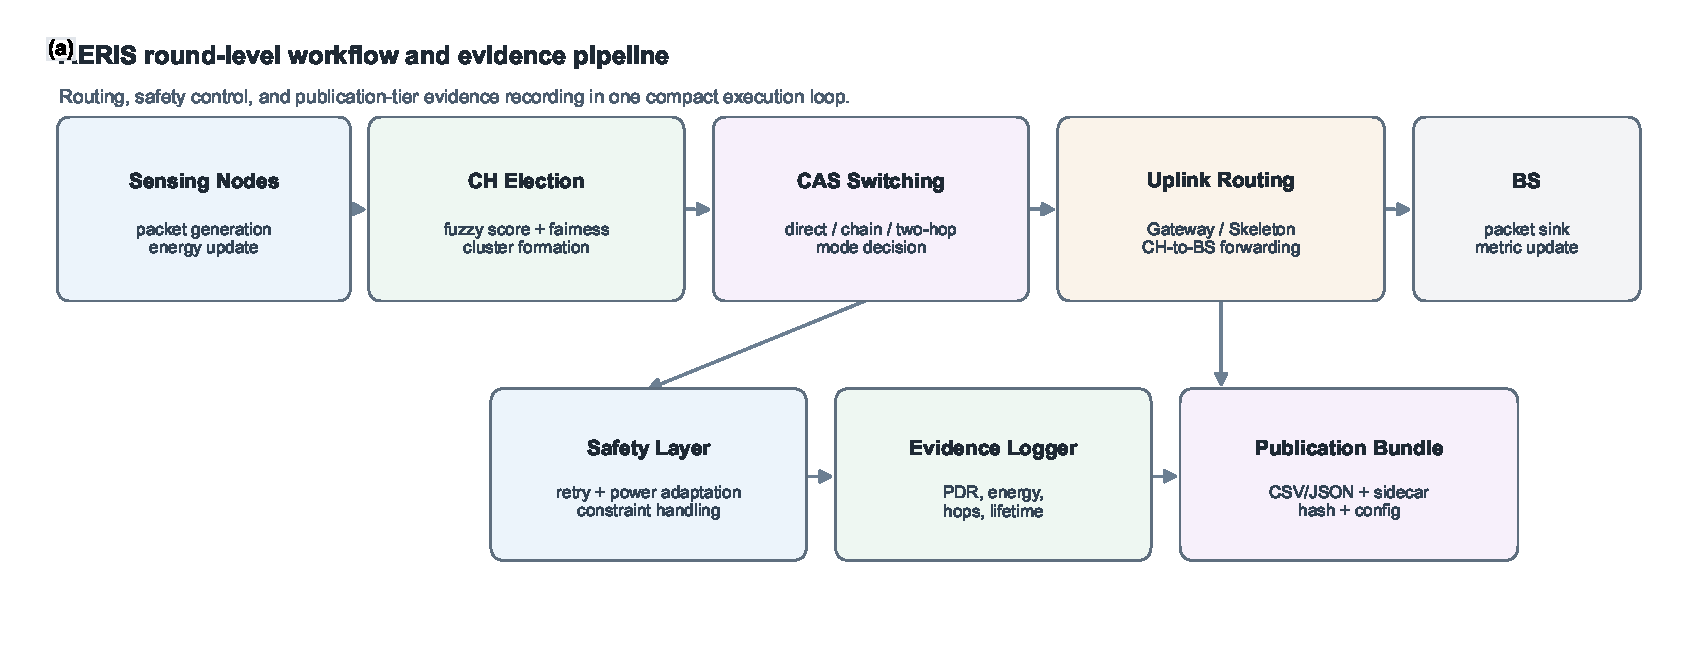
\includegraphics[width=0.98\textwidth]{fig0_aeris_workflow_20260228_s81.pdf}
\caption{Three-phase AERIS workflow from per-round control decisions to evidence output. The diagram separates routing decisions, safety control, and metric/provenance logging to keep reproducibility boundaries explicit.}
\label{fig:aeris_workflow}
\end{figure}

\section{Experimental Setup}
\subsection{Publication-Tier Settings}
\begin{itemize}
\item Simulator: Python implementation with logged provenance.
\item Channel environments: indoor\_office, indoor\_factory, outdoor\_urban, outdoor\_suburban.
\item Default node count: 100.
\item Seeds for multi-environment and ablation: 30 independent seeds.
\item Seeds for scalability: primary large-scale matrix with n=3200 per environment-node-protocol cell (100--1000 nodes, 4 environments; strict-physics flags enabled).
\item Baselines: LEACH, PEGASIS, HEED, TEEN.
\end{itemize}

\subsection{Evidence Scope}
The analysis is grounded in publication-tier multi-environment comparison, ablation, scalability, hop-based latency, energy-lifetime statistics, and NS-3 trend validation. Cross-regime numerical pooling is avoided.

\subsection{Fairness Controls and Simulator Credibility}
The simulator is custom Python code, so fairness controls are explicitly enforced in publication-tier runs:
\begin{itemize}
\item identical tx-power configuration across protocols in the same matrix,
\item identical environment taxonomy and node-scale grid per protocol,
\item deterministic seed schedules per regime,
\item no reliability override (\texttt{force\_ctp\_reliable=False}).
\end{itemize}

To reduce implementation-bias risk, the primary large-scale matrix removes previously identified baseline suppressors and reruns the four-environment scalability matrix under explicit collision and relay settings. NS-3 is then used as an independent trend-level check for AERIS versus LEACH under aligned environment definitions. NS-3 is therefore used as external directional validation rather than as a one-to-one numerical replacement of the Python matrix.

\subsection{Simulator Regimes and Physics Assumptions}
This study reports two regime tiers for scalability interpretation. The primary tier is the large-scale matrix (explicit collision-and-relay settings, balanced n=3200 per cell) and is used for large-scale ranking claims. The secondary tier (stress and sensitivity blocks) is retained for matched stress comparison (patch minus control) and tx-power diagnostics, not for replacing the primary ranking matrix.

\begin{table}[H]
\caption{Evidence-regime map used in this manuscript.}
\label{tab:regime_map}
\centering
\resizebox{\linewidth}{!}{
\begin{tabular}{llll}
\toprule
Block & Scope & Typical sample size & Role in claims \\
\midrule
100-node matrix & 4 env $\times$ 5 protocols & n=30 per env-protocol cell & Core reliability comparison \\
Primary large-scale matrix & 4 env $\times$ 6 node counts $\times$ 5 protocols & n=3200 per env-node-protocol cell & Primary large-scale evidence \\
Stress block A (stress comparison, patch-control) & 4 env $\times$ 6 node counts $\times$ 5 protocols & patch n=1000, control n=600 & Physics-stress calibration \\
Sensitivity block (tx-power matrix) & 4 env $\times$ 3 tx levels $\times$ 6 node counts $\times$ 5 protocols & n=1000 per env-node-protocol cell & Tx-power boundary analysis \\
Stress block B (matched stress comparison) & 4 env $\times$ 6 node counts $\times$ 5 protocols & patch n=1000, control n=1000 & Matched strict-physics confirmation \\
NS-3 alignment & 4 env $\times$ 7 node counts, AERIS vs LEACH & n=30 per env-node-protocol cell & Trend-level cross-platform check \\
\bottomrule
\end{tabular}
}
\end{table}

Table~\ref{tab:regime_map} defines the claim boundary used throughout the Results and Discussion sections.

\subsection{Statistical Methods}
For pairwise protocol comparisons, we use Welch's two-sample $t$-test:
\begin{equation}
t=\frac{\bar{x}_1-\bar{x}_2}{\sqrt{\frac{s_1^2}{n_1}+\frac{s_2^2}{n_2}}},
\end{equation}
because variance equality is not assumed across protocols and environments. Family-wise error control is handled by Holm correction within each reported comparison family. Effect size is reported with Hedges' $g$:
\begin{equation}
g = J\cdot\frac{\bar{x}_1-\bar{x}_2}{s_p},\quad
J=1-\frac{3}{4(n_1+n_2)-9},
\end{equation}
and interpreted as small (0.2), medium (0.5), and large (0.8) in absolute value. Confidence intervals are reported as two-sided 95\% intervals. All significance statements in this manuscript are based on Holm-corrected $p$ values. For large-$n$ cells, interpretation is based jointly on corrected $p$ values, effect size, and absolute PDR delta. Reported table-wise standard deviations are treated as descriptive values from the corresponding result files; inferential conclusions are computed from raw replicate-level records.

\subsection{Reproducibility Controls}
All publication-tier scripts in this study use deterministic seed lists and disable reliability-override logic. This guarantees that PDR reflects simulated delivery behavior rather than forced delivery assumptions. We treat hop count as a latency proxy, not a wall-clock latency measurement. Significance statements are accepted only when consistent with the declared regime-specific sample size.

\subsection{Auditability Constraints}
To keep claims machine-checkable, each publication-tier output includes run-tier tags, metric tags, and script/hash sidecar metadata. Claims in the main text are restricted to matrices that satisfy declared sample-size and metric constraints. This prevents mixing exploratory diagnostics with publication-tier statements.

\section{Results}
\subsection{Multi-Environment Comparison at 100 Nodes (n=30)}
\begin{table}[H]
\caption{Legacy comparability matrix (strict collision/relay flags disabled): PDR by environment at 100 nodes (n=30 per environment-protocol cell). Values are shown at 4-decimal precision; minor last-digit differences come from rounding conventions in source records.}
\label{tab:pdr100}
\centering
\resizebox{\linewidth}{!}{
\begin{tabular}{lccccc}
\toprule
Environment & AERIS & LEACH & PEGASIS & HEED & TEEN \\
\midrule
indoor\_office   & 0.9739$\pm$0.0047 & 0.5543$\pm$0.0401 & 0.9078$\pm$0.0166 & 0.9371$\pm$0.0076 & 0.8222$\pm$0.0044 \\
indoor\_factory  & 0.6031$\pm$0.0258 & 0.1614$\pm$0.0209 & 0.1928$\pm$0.0255 & 0.2326$\pm$0.0263 & 0.3113$\pm$0.0245 \\
outdoor\_urban   & 0.3745$\pm$0.0354 & 0.0552$\pm$0.0127 & 0.0542$\pm$0.0117 & 0.0635$\pm$0.0121 & 0.1201$\pm$0.0183 \\
outdoor\_suburban& 0.7451$\pm$0.0193 & 0.2703$\pm$0.0272 & 0.3382$\pm$0.0329 & 0.4221$\pm$0.0313 & 0.4752$\pm$0.0236 \\
\bottomrule
\end{tabular}
}
\end{table}
All pairwise AERIS-versus-baseline comparisons in Table~\ref{tab:pdr100} are significant after Holm correction ($p<0.001$).

At 100 nodes, AERIS ranks first in all four tested environments within the evaluated baseline set (LEACH, PEGASIS, HEED, and TEEN). This claim is restricted to the 100-node matrix and should not be generalized to the 1000-node regime.
Because Table~\ref{tab:pdr100} is generated from the legacy 100-node regime (without strict collision/relay flags), its absolute values are intentionally not pooled with the primary large-scale matrix.

\begin{figure}[H]
\centering
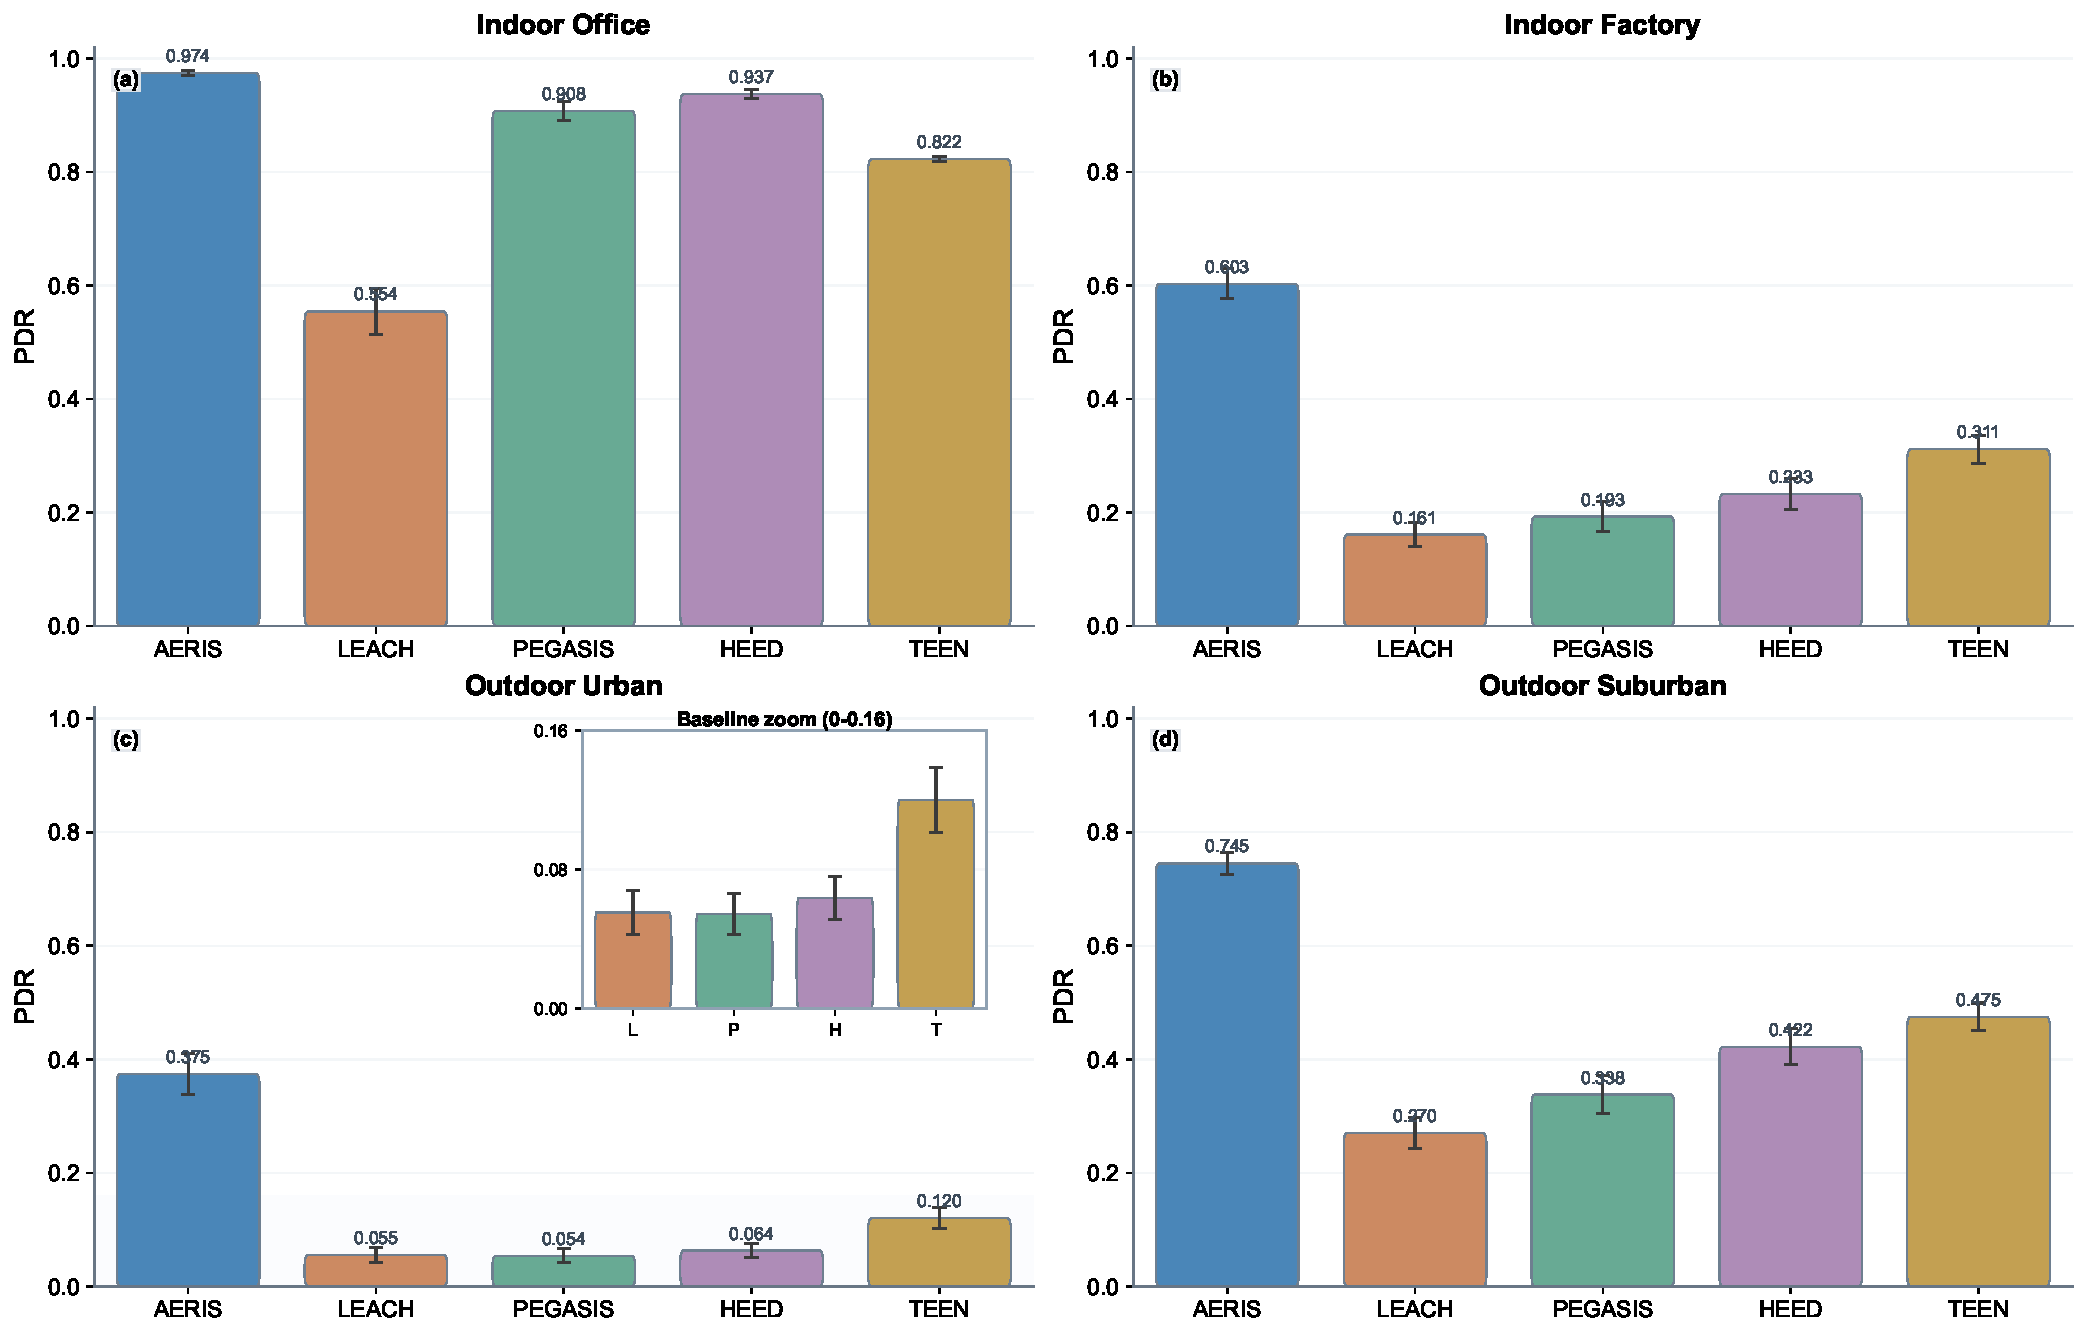
\includegraphics[width=0.99\textwidth]{fig1_env_pdr_panel_20260228_s81.pdf}
\caption{PDR comparison panel at 100 nodes (4 environments, n=30). The outdoor\_urban panel includes a baseline-only inset (0--0.16 PDR; LEACH/PEGASIS/HEED/TEEN) to avoid visual duplication while preserving the global 0--1 y-axis in the main panel.}
\label{fig:env_panel}
\end{figure}

Figure~\ref{fig:env_panel} visually confirms the cross-environment ordering reported in Table~\ref{tab:pdr100}.

\subsection{Ablation: Environment-Dependent Effects (n=30)}
\begin{table}[H]
\caption{Full vs no\_gateway PDR (mean $\pm$ std, reported at 4-decimal precision).}
\label{tab:ablation_gateway}
\centering
\begin{tabular}{lccc}
\toprule
Environment & Full & no\_gateway & Delta (no\_gateway - full) \\
\midrule
indoor\_office    & 0.9739$\pm$0.0047 & 0.9741$\pm$0.0036 & +0.0002 \\
indoor\_factory   & 0.6031$\pm$0.0258 & 0.5806$\pm$0.0215 & -0.0225 \\
outdoor\_urban    & 0.3745$\pm$0.0354 & 0.3534$\pm$0.0301 & -0.0212 \\
outdoor\_suburban & 0.7451$\pm$0.0193 & 0.7306$\pm$0.0264 & -0.0146 \\
\bottomrule
\end{tabular}
\end{table}

Gateway is positive in three environments and near-neutral in indoor\_office. CAS is not consistently positive across environments.
In indoor\_office, the Full-vs-no\_gateway gap is +0.0002 (absolute PDR), so this cell is treated as practically neutral.
These effects are quantified in Table~\ref{tab:ablation_gateway}.

\begin{figure}[H]
\centering
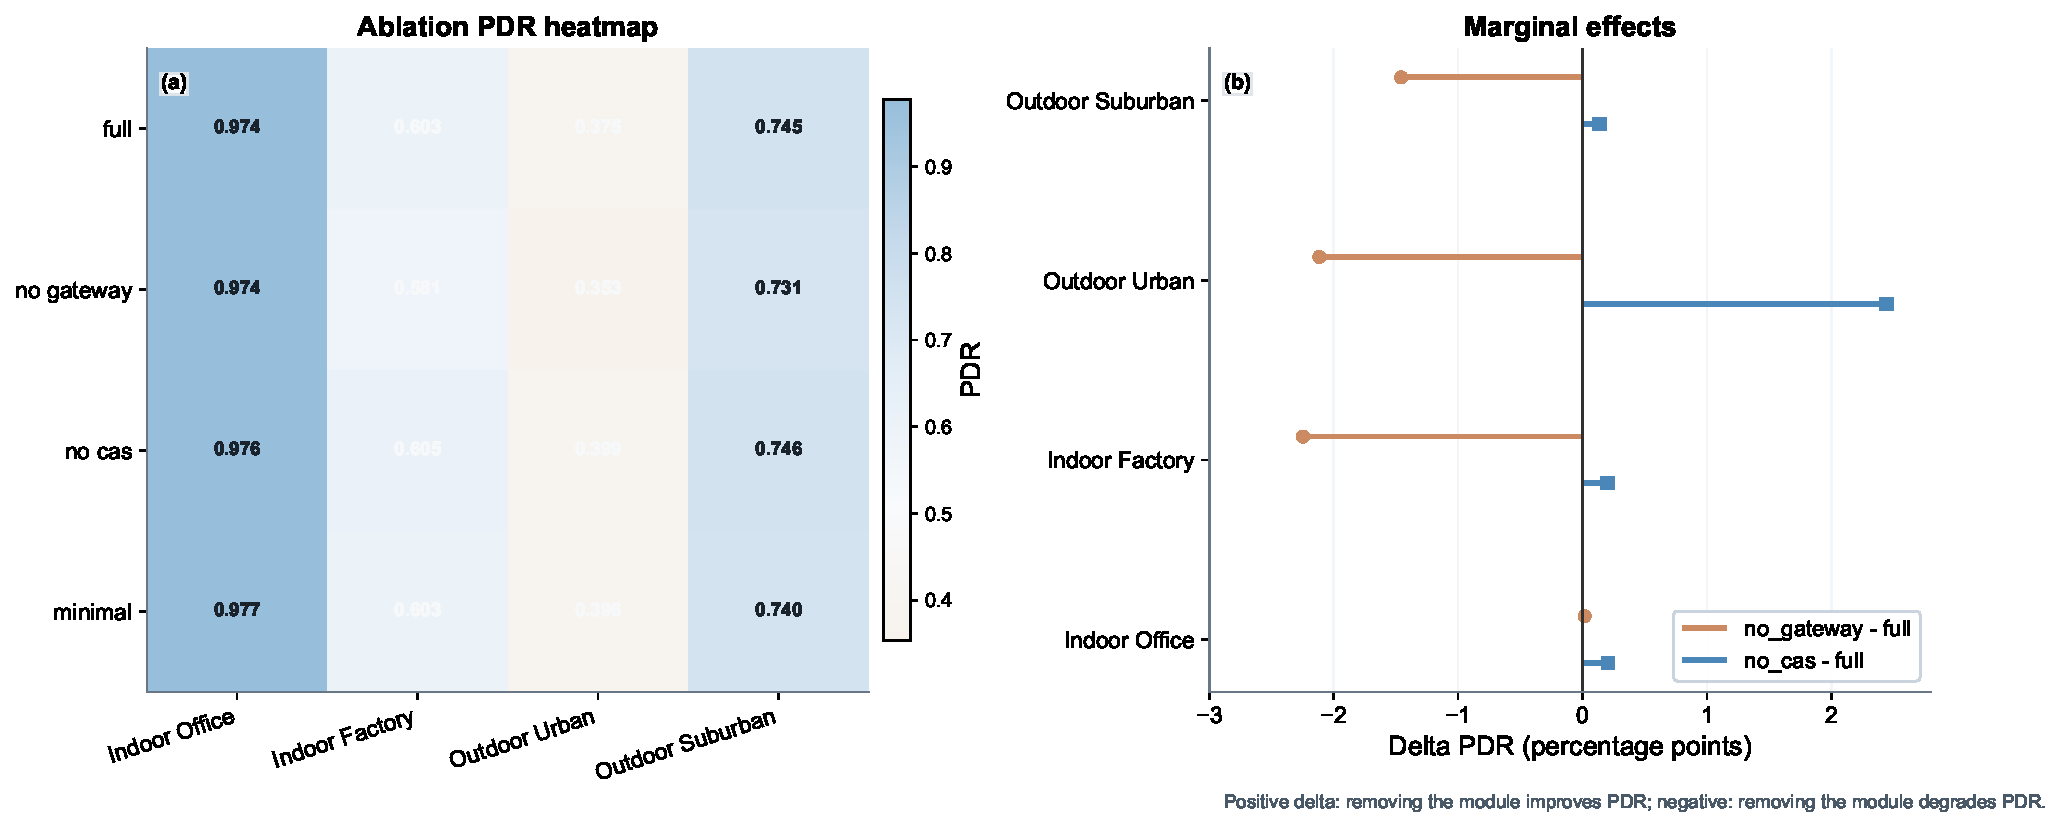
\includegraphics[width=0.99\textwidth]{fig2_ablation_panel_20260228_s81.pdf}
\caption{Ablation panel: heatmap and marginal effects (n=30).}
\label{fig:ablation_panel}
\end{figure}

Figure~\ref{fig:ablation_panel} highlights the environment dependence of gateway and CAS contributions.

\subsection{Scalability (100--1000 Nodes; Balanced n=3200 per Cell)}
\begin{table}[H]
\caption{PDR ranking at 1000 nodes from the primary large-scale matrix (n=3200 per cell).}
\label{tab:scale1000}
\centering
\begin{tabular}{lcccccc}
\toprule
Environment & AERIS & LEACH & PEGASIS & HEED & TEEN & AERIS rank \\
\midrule
indoor\_office    & 0.6771 & 0.0282 & 0.9884 & 0.0134 & 0.0170 & 2nd \\
indoor\_factory   & 0.7284 & 0.0108 & 0.2999 & 0.0054 & 0.0070 & 1st \\
outdoor\_urban    & 0.1359 & 0.0041 & 0.0987 & 0.0016 & 0.0025 & 1st \\
outdoor\_suburban & 0.7275 & 0.0160 & 0.4725 & 0.0088 & 0.0106 & 1st \\
\bottomrule
\end{tabular}
\end{table}

AERIS is first in three environments at 1000 nodes (indoor\_factory, outdoor\_urban, outdoor\_suburban) and second in indoor\_office where PEGASIS remains dominant (Table~\ref{tab:scale1000}).
Across the full 24-cell matrix (4 environments $\times$ 6 node counts), AERIS ranks first in 18 cells and PEGASIS ranks first in the 6 indoor\_office cells.
Unlike the legacy 100-node comparability matrix, the primary large-scale matrix shows physically plausible scale behavior: AERIS PDR decreases from 100 to 1000 nodes in all four environments under explicit collision and relay constraints.

\subsection{Statistical Robustness Snapshot (AERIS vs Strongest Baseline)}
\begin{table}[H]
\caption{Holm-corrected significance snapshot at 1000 nodes (AERIS vs strongest baseline in each environment).}
\label{tab:robust_snapshot}
\centering
\begin{tabular}{lcccccc}
\toprule
Environment & Nodes & $\Delta$PDR & Hedges' $g$ & Holm $p$ & Significant \\
\midrule
indoor\_office    & 1000 & -0.311272 (vs PEGASIS) & -14.2041 & $<10^{-300}$ & yes \\
indoor\_factory   & 1000 & +0.428522 (vs PEGASIS) & +5.0292 & $<10^{-300}$ & yes \\
outdoor\_urban    & 1000 & +0.037265 (vs PEGASIS) & +0.5592 & $8.43\times10^{-107}$ & yes \\
outdoor\_suburban & 1000 & +0.255009 (vs PEGASIS) & +2.8235 & $<10^{-300}$ & yes \\
\bottomrule
\end{tabular}
\end{table}

This snapshot shows positive AERIS deltas in three harsh environments and a negative delta in indoor\_office, where PEGASIS is the strongest baseline at large scale.
The corresponding statistics are reported in Table~\ref{tab:robust_snapshot}.
For very large sample sizes, practical interpretation in this study still follows both effect size and absolute PDR gap rather than significance labels alone.
The very large absolute values of Hedges' $g$ in harsh environments reflect both large mean gaps and low within-group variance under large sample sizes; they should be interpreted as magnitude indicators within this experiment design, not as cross-study constants.\footnote{For large-\(n\) comparisons with very small within-group variance, standardized effect sizes can become extremely large. In this manuscript, Hedges' \(g\) is therefore interpreted jointly with absolute \(\Delta\)PDR and confidence intervals, not as a stand-alone cross-study scale.}

\begin{figure}[H]
\centering
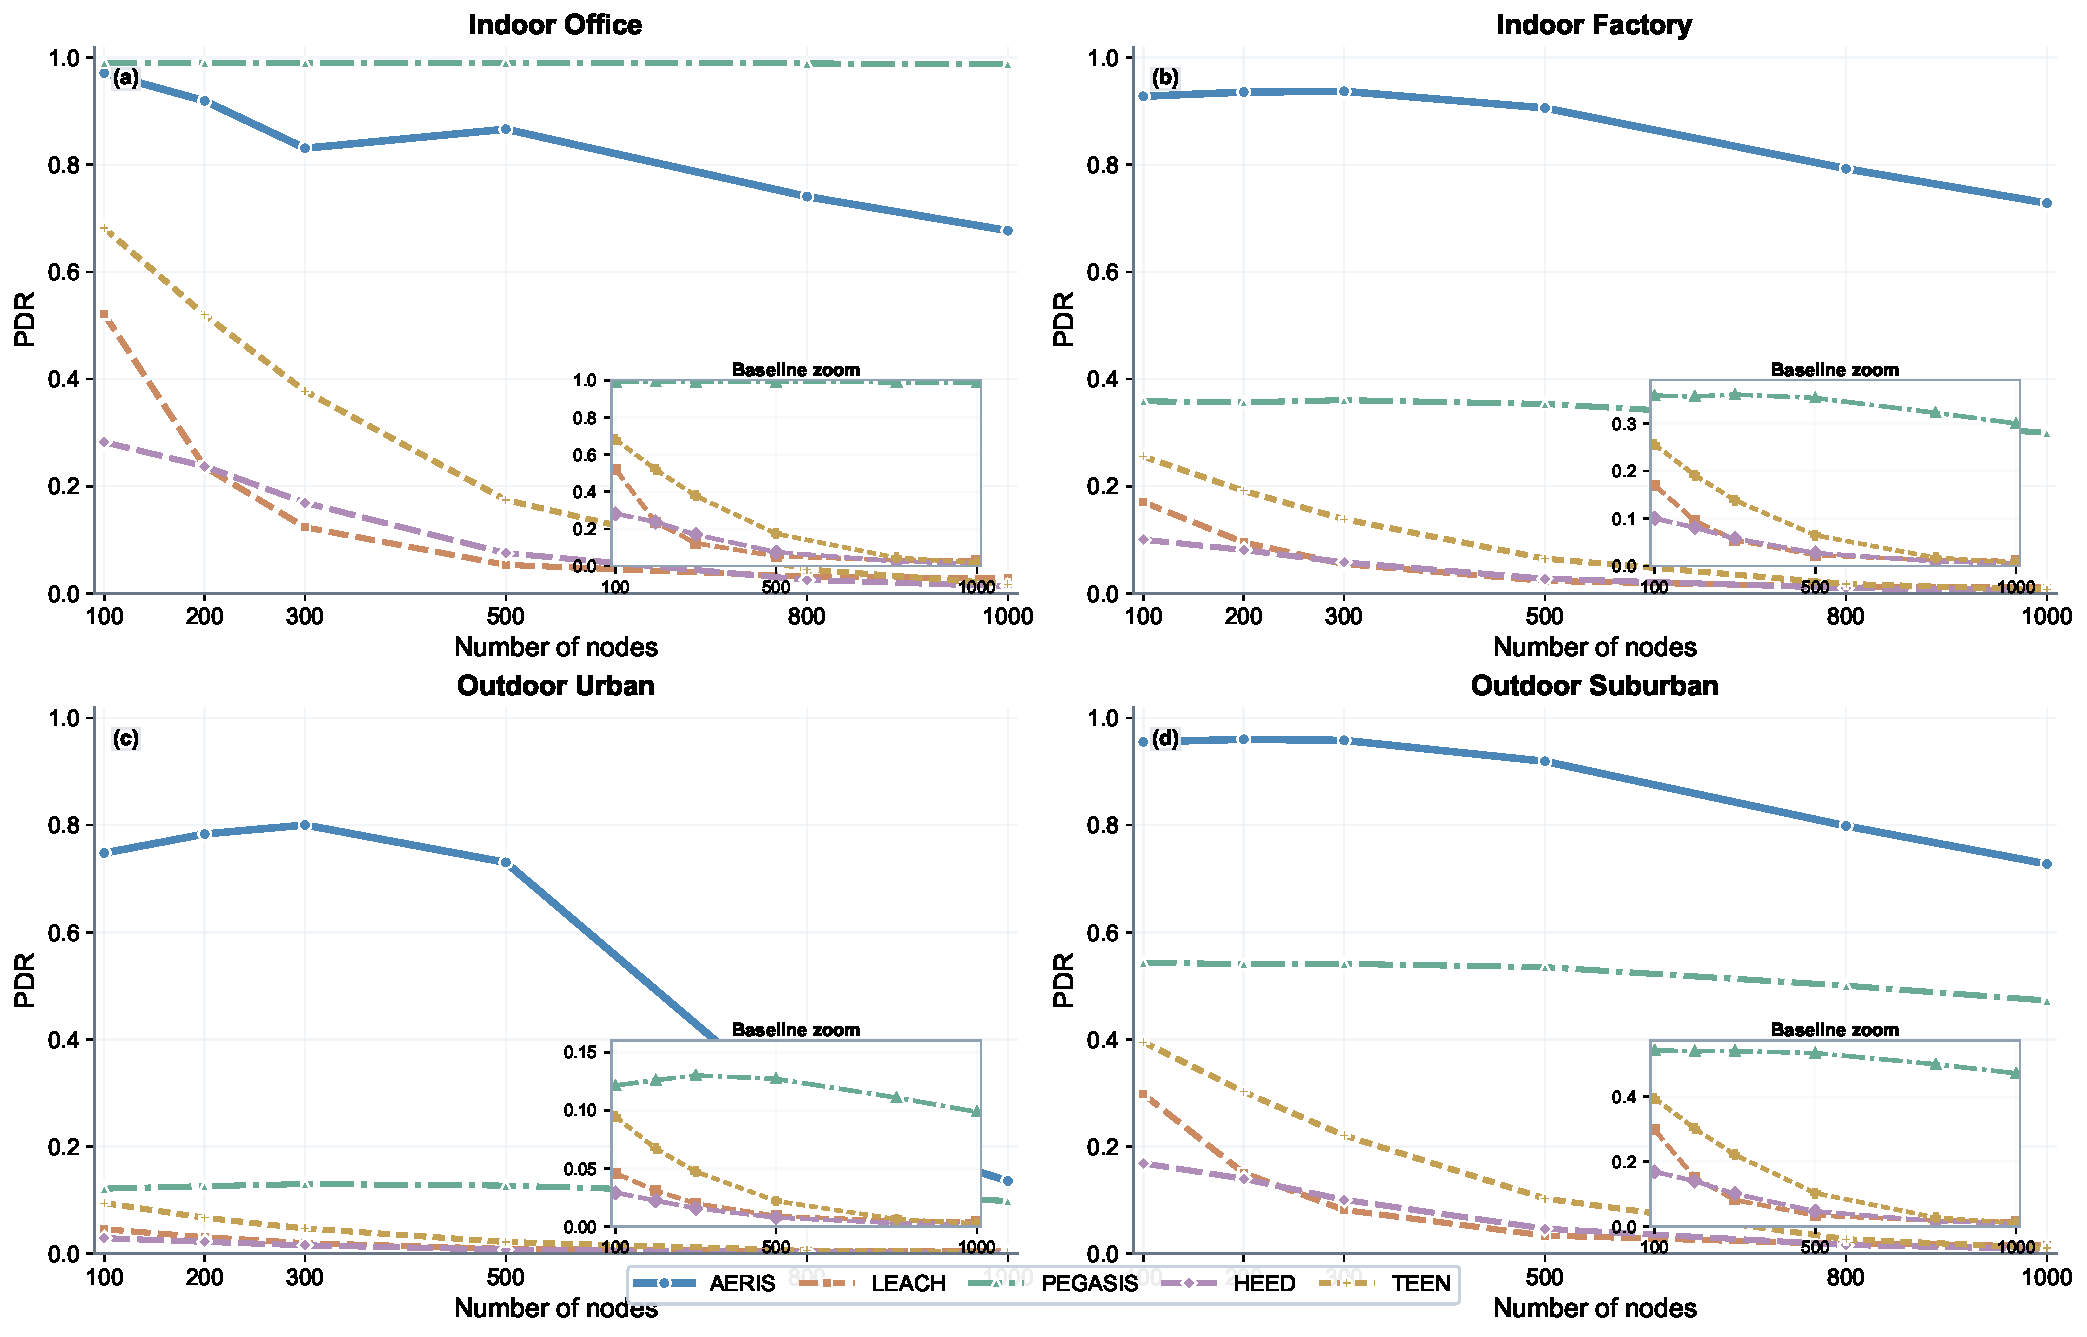
\includegraphics[width=0.99\textwidth]{fig3_scalability_panel_20260228_s81.pdf}
\caption{Primary large-scale scalability trends (n=3200 per cell, 95\% CI bands). Each panel includes all five protocols over six node counts on a common 0--1 y-axis; a baseline zoom inset is added per environment to make low-PDR protocol separation readable under the shared global axis.}
\label{fig:scalability_panel}
\end{figure}

Figure~\ref{fig:scalability_panel} together with Table~\ref{tab:robust_snapshot} provides the trend-and-significance view of the primary large-scale matrix.

\subsection{Rigor-Patch Pilot Sanity Check (n=60)}
To test simulator-physics consistency before the full rerun, we ran a local pilot with collision and baseline multi-hop relay enabled, using the same environment taxonomy and nodes \{100, 500, 1000\} with n=60 per cell. This pilot is retained as a diagnostic snapshot and is not used in primary claim tables.

\begin{table}[H]
\caption{AERIS PDR under the rigor-patch pilot (n=60 per environment-node cell). This pilot table is included for regime-transition diagnostics and is not used for primary claims.}
\label{tab:rigor_patch}
\centering
\begin{tabular}{lccc}
\toprule
Environment & 100 nodes & 500 nodes & 1000 nodes \\
\midrule
indoor\_office    & 0.9706 & 0.8676 & 0.6746 \\
indoor\_factory   & 0.9283 & 0.9083 & 0.7355 \\
outdoor\_urban    & 0.7487 & 0.7362 & 0.1492 \\
outdoor\_suburban & 0.9563 & 0.9193 & 0.7307 \\
\bottomrule
\end{tabular}
\end{table}

The key pilot observation is monotonicity recovery: AERIS PDR decreases with scale in all four environments. In indoor\_office, PEGASIS is higher than AERIS under this stricter setting, while AERIS remains clearly higher in the other three environments. The pilot therefore served as a gate check for launching the full primary large-scale matrix and is reported only for diagnostic completeness.
The pilot values summarized above are reported in Table~\ref{tab:rigor_patch}.

\subsection{Stress-Comparison Matrix (Four Environments)}
To reduce seed and sampling confounders, we ran Stress block A (patch-minus-control comparison) in all four environments (indoor\_office, indoor\_factory, outdoor\_urban, and outdoor\_suburban). The patch mode enables collision and baseline relay mechanisms; the control mode uses the legacy control configuration. Patch cells use n=1000 and control cells use n=600.

\begin{table}[H]
\caption{AERIS PDR in Stress block A (patch-minus-control comparison, four environments). The two curves correspond to patch/control executions under the same environment and node settings.}
\label{tab:s9_patch_control}
\centering
\begin{tabular}{lccc}
\toprule
Environment & Nodes & Patch & Control \\
\midrule
indoor\_office & 100  & 0.9714 & 0.9948 \\
indoor\_office & 500  & 0.8679 & 0.9902 \\
indoor\_office & 1000 & 0.6779 & 0.9899 \\
indoor\_factory & 100  & 0.9281 & 0.9329 \\
indoor\_factory & 500  & 0.9060 & 0.9627 \\
indoor\_factory & 1000 & 0.7291 & 0.9726 \\
outdoor\_urban & 100  & 0.7482 & 0.7559 \\
outdoor\_urban & 500  & 0.7299 & 0.8460 \\
outdoor\_urban & 1000 & 0.1372 & 0.8845 \\
outdoor\_suburban & 100  & 0.9556 & 0.9744 \\
outdoor\_suburban & 500  & 0.9198 & 0.9859 \\
outdoor\_suburban & 1000 & 0.7280 & 0.9897 \\
\bottomrule
\end{tabular}
\end{table}

Table~\ref{tab:s9_patch_control} provides the stress-comparison baseline (patch minus control) used for cross-regime interpretation.

Three observations are robust in this stress comparison matrix. First, AERIS remains above LEACH/HEED/TEEN under patch mode in all four environments at 1000 nodes. Second, PEGASIS is minimally affected by the patch, with near-zero deltas and non-significant tests in all 24 PEGASIS cells\footnote{Across the 24 PEGASIS cells in this stress comparison matrix, \(|\Delta_{\text{patch-control}}| \le 0.0044\), all Holm-adjusted \(p\)-values are \(1.0000\), and \(\max |g| = 0.0903\), consistent with a near-zero effect.}. A technical hypothesis is that serialized chain forwarding in PEGASIS exposes fewer branch decisions to the patch toggles than cluster-centric protocols, so fewer control points are perturbed under the current implementation path. Third, AERIS patch-minus-control deltas are significant in all 24 AERIS cells after Holm correction, with the largest absolute drop in outdoor\_urban at high scale. Table~\ref{tab:s9_pegasis_1000} provides the 1000-node PEGASIS snapshot supporting this interpretation.

In the matched stress-confirmation matrix, PEGASIS shows exact zero deltas in indoor\_factory (all six node counts). We treat this as an implementation-coupling anomaly requiring dedicated implementation audit, not as physical invariance evidence. The patch can also be overly aggressive for baseline paths at high scale, so this block is interpreted as stress evidence rather than as a final replacement matrix. To remove sample-size asymmetry from Stress block A, we run this matched stress-confirmation matrix (patch \(n=1000\), control \(n=1000\) per cell) and report it separately below.

Consistency between the stress comparison matrix and the matched confirmation matrix is assessed from the matched-delta tables and significance files; both matrices preserve the same direction pattern for AERIS across environment-scale cells.

\begin{table}[H]
\caption{PEGASIS patch-versus-control snapshot at 1000 nodes from the stress comparison matrix (n=1000 patch, n=600 control).}
\label{tab:s9_pegasis_1000}
\centering
\begin{tabular}{lcccc}
\toprule
Environment & Delta (patch-control) & Hedges' $g$ & Holm $p$ & Significant \\
\midrule
indoor\_office    & -0.0003 & -0.0435 & 1.0000 & No \\
indoor\_factory   & +0.0006 & +0.0057 & 1.0000 & No \\
outdoor\_urban    & +0.0017 & +0.0252 & 1.0000 & No \\
outdoor\_suburban & -0.0011 & -0.0085 & 1.0000 & No \\
\bottomrule
\end{tabular}
\end{table}

\subsection{TX-Power Sensitivity Block (Four Environments)}
We additionally evaluate tx-power sensitivity under the upgraded simulation path by comparing \SI{5}{dBm}, \SI{10}{dBm}, and \SI{15}{dBm} across four environments, six node counts (100, 200, 300, 500, 800, 1000), and five protocols (n=1000 per cell). The full pairwise matrix contains 360 matched comparisons (4 environments $\times$ 6 node counts $\times$ 5 protocols $\times$ 3 pairwise tx comparisons), and all 360 are significant after Holm correction.

\begin{table}[H]
\caption{AERIS power-sensitivity snapshot at 1000 nodes (mean PDR, tx5/tx10/tx15) from the power-sensitivity matrix (n=1000 per cell).}
\label{tab:s10_aeris_1000}
\centering
\begin{tabular}{lccccc}
\toprule
Environment & tx=\SI{5}{dBm} & tx=\SI{10}{dBm} & tx=\SI{15}{dBm} & Delta (5--10) & Delta (5--15) \\
\midrule
indoor\_office    & 0.8176 & 0.6775 & 0.5404 & +0.1401 & +0.2771 \\
indoor\_factory   & 0.6633 & 0.7291 & 0.5032 & -0.0658 & +0.1601 \\
outdoor\_urban    & 0.0582 & 0.1363 & 0.1634 & -0.0781 & -0.1052 \\
outdoor\_suburban & 0.7679 & 0.7269 & 0.5431 & +0.0411 & +0.2249 \\
\bottomrule
\end{tabular}
\end{table}

Table~\ref{tab:s10_aeris_1000} reports the 1000-node AERIS tx-power snapshot used in this subsection.

\begin{figure}[H]
\centering
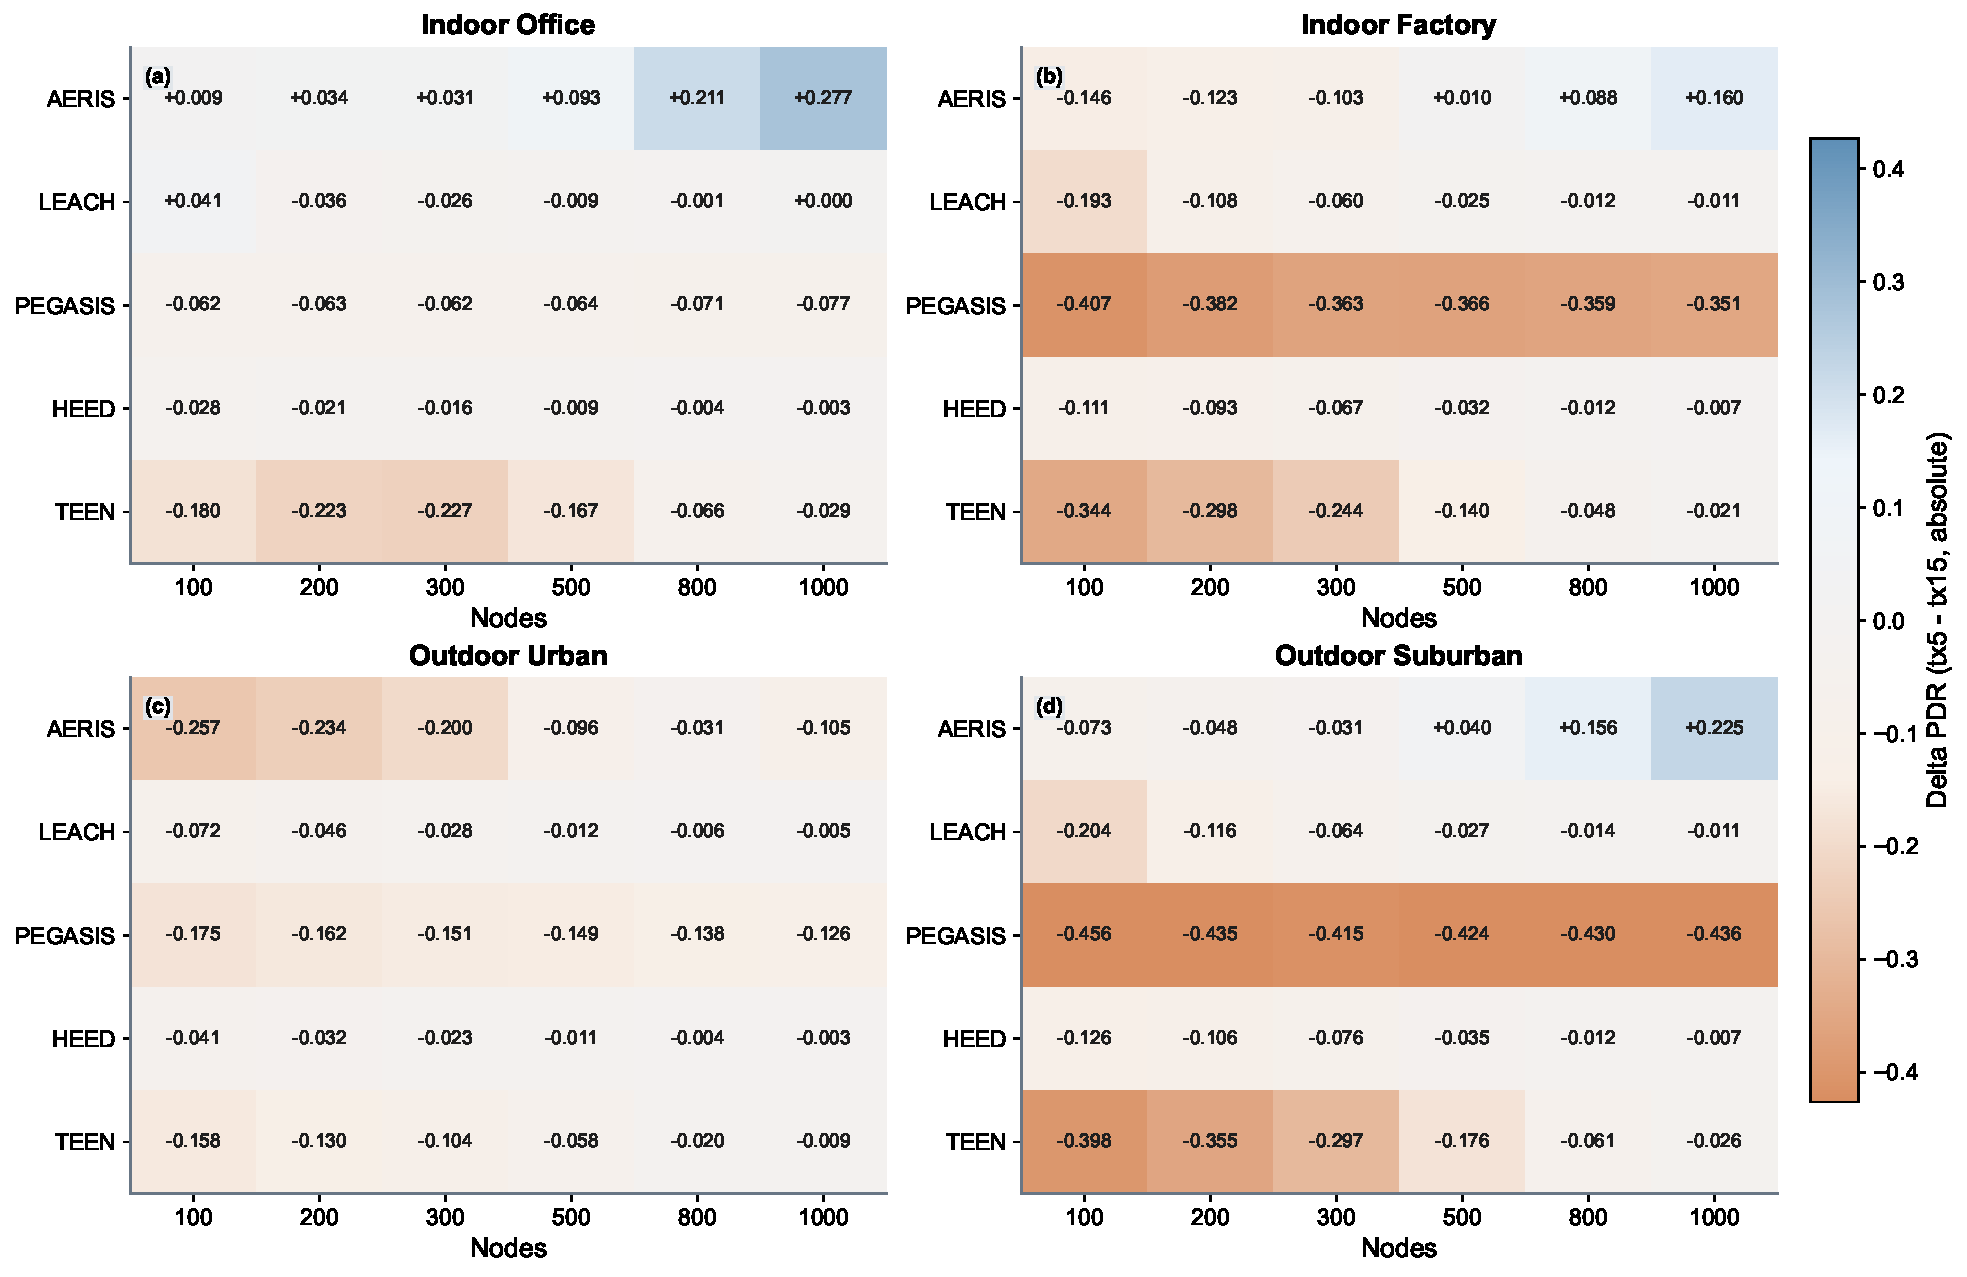
\includegraphics[width=0.99\textwidth]{fig6_s10_delta_maps_20260228_s81.pdf}
\caption{Power-sensitivity delta maps (\(\Delta\)PDR = tx5 $-$ tx15, absolute PDR units; 4 environments $\times$ 5 protocols $\times$ 6 node counts = 120 cells). No cells are filtered. Cross markers denote Holm non-significant cells.}
\label{fig:s10_power_sensitivity}
\end{figure}

\begin{figure}[H]
\centering
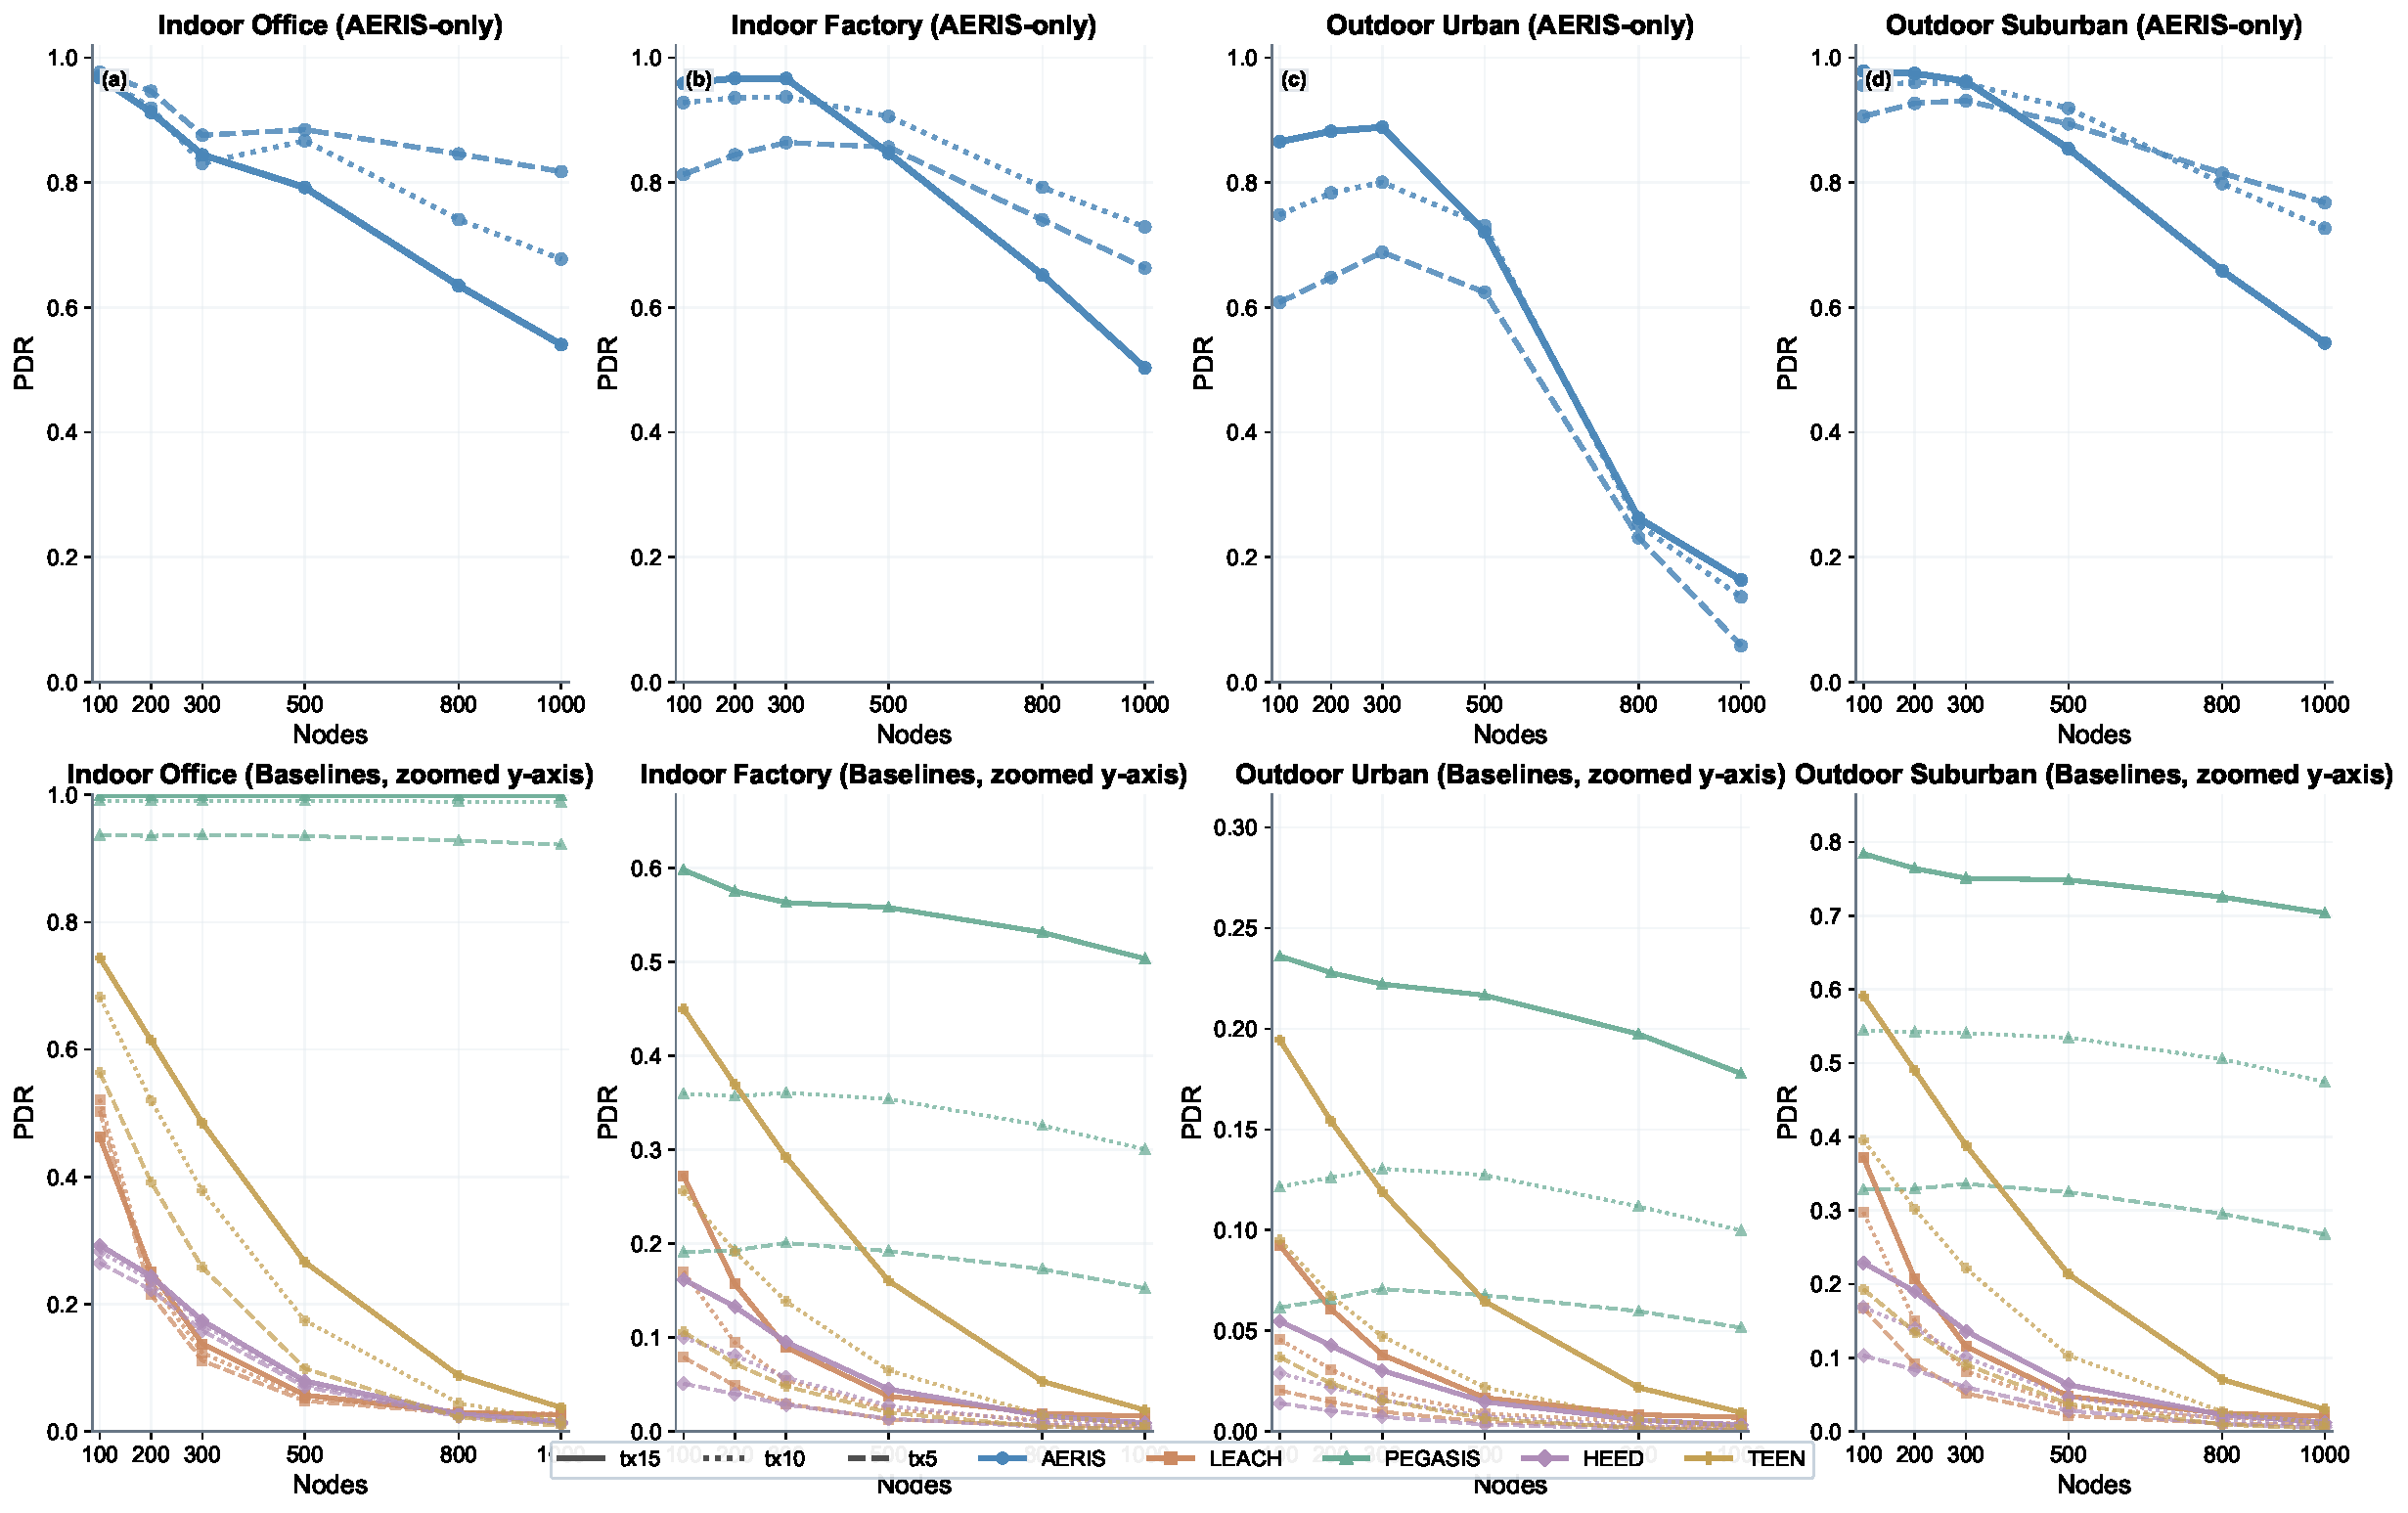
\includegraphics[width=0.99\textwidth]{fig10_s10_absolute_profiles_20260228_s81.pdf}
\caption{Absolute PDR profiles from the power-sensitivity matrix. Top row: AERIS (line style = tx level, common y-axis 0--1). Bottom row: baseline protocols with environment-specific y-axis zoom for low-PDR readability.}
\label{fig:s10_absolute_profiles}
\end{figure}

The tx-power block confirms that response is environment-dependent and non-monotonic under the current routing and channel settings. In particular, raising tx-power does not guarantee higher PDR in every environment-node cell. A plausible mechanism is interference-domain expansion: higher transmit power increases both reachable receivers and competing transmitters, which can increase collision probability in dense regimes and partially offset link-budget gains. In the completed power-sensitivity matrix, all 360 pairwise tx comparisons are significant after Holm correction.
Two targeted cells are highlighted because they are easy to misread under a monotonicity assumption. First, indoor\_factory at 500 nodes follows tx10 $>$ tx5 $>$ tx15 for AERIS (0.9060, 0.8569, 0.8471), so the local optimum is mid-power rather than high-power. Second, outdoor\_urban at 800 nodes shows high dispersion for AERIS (CV$_{\text{tx5}}=0.54$, CV$_{\text{tx10}}=0.44$, CV$_{\text{tx15}}=0.34$), indicating a near-threshold regime where connectivity and collision states alternate across replicates. This variance concentration at high scale is consistent with intermittent percolation behavior in sparse urban connectivity, where small contention shifts can move rounds between connected and fragmented states.
Figures~\ref{fig:s10_power_sensitivity} and~\ref{fig:s10_absolute_profiles} are interpreted together with Table~\ref{tab:s10_aeris_1000} to avoid delta-only bias.

\subsection{Matched Stress Comparison Confirmation Matrix (Four Environments, n=1000 vs 1000)}
To remove remaining sample-size asymmetry from Stress block A, we completed a fully matched stress-comparison matrix in which both patch and control arms use n=1000 per environment-node-protocol cell (4 environments $\times$ 6 node counts $\times$ 5 protocols). This matrix directly tests whether stricter physics assumptions improve or degrade reliability under matched sampling.

\begin{table}[H]
\caption{AERIS patch-minus-control deltas in the matched stress-confirmation matrix (delta = patch - control).}
\label{tab:s11_aeris_delta}
\centering
\begin{tabular}{lcc}
\toprule
Environment & Delta at 100 nodes & Delta at 1000 nodes \\
\midrule
indoor\_office    & -0.0234 & -0.3120 \\
indoor\_factory   & -0.0052 & -0.2435 \\
outdoor\_urban    & -0.0077 & -0.7474 \\
outdoor\_suburban & -0.0191 & -0.2616 \\
\bottomrule
\end{tabular}
\end{table}

Table~\ref{tab:s11_aeris_delta} summarizes the AERIS matched-delta boundary in the confirmation matrix.

In the matched matrix, AERIS patch-minus-control deltas are negative and significant in all 24 environment-scale cells after Holm correction (24/24 significant; Hedges' $g$ range: -0.47 to -15.36). Therefore, under the current patch configuration (\texttt{mac-collision + multihop-relay}), stricter physics assumptions reduce reliability rather than increase it. This means the stress block is evidence for realism stress, not yet evidence for superior calibrated performance.

\begin{figure}[H]
\centering
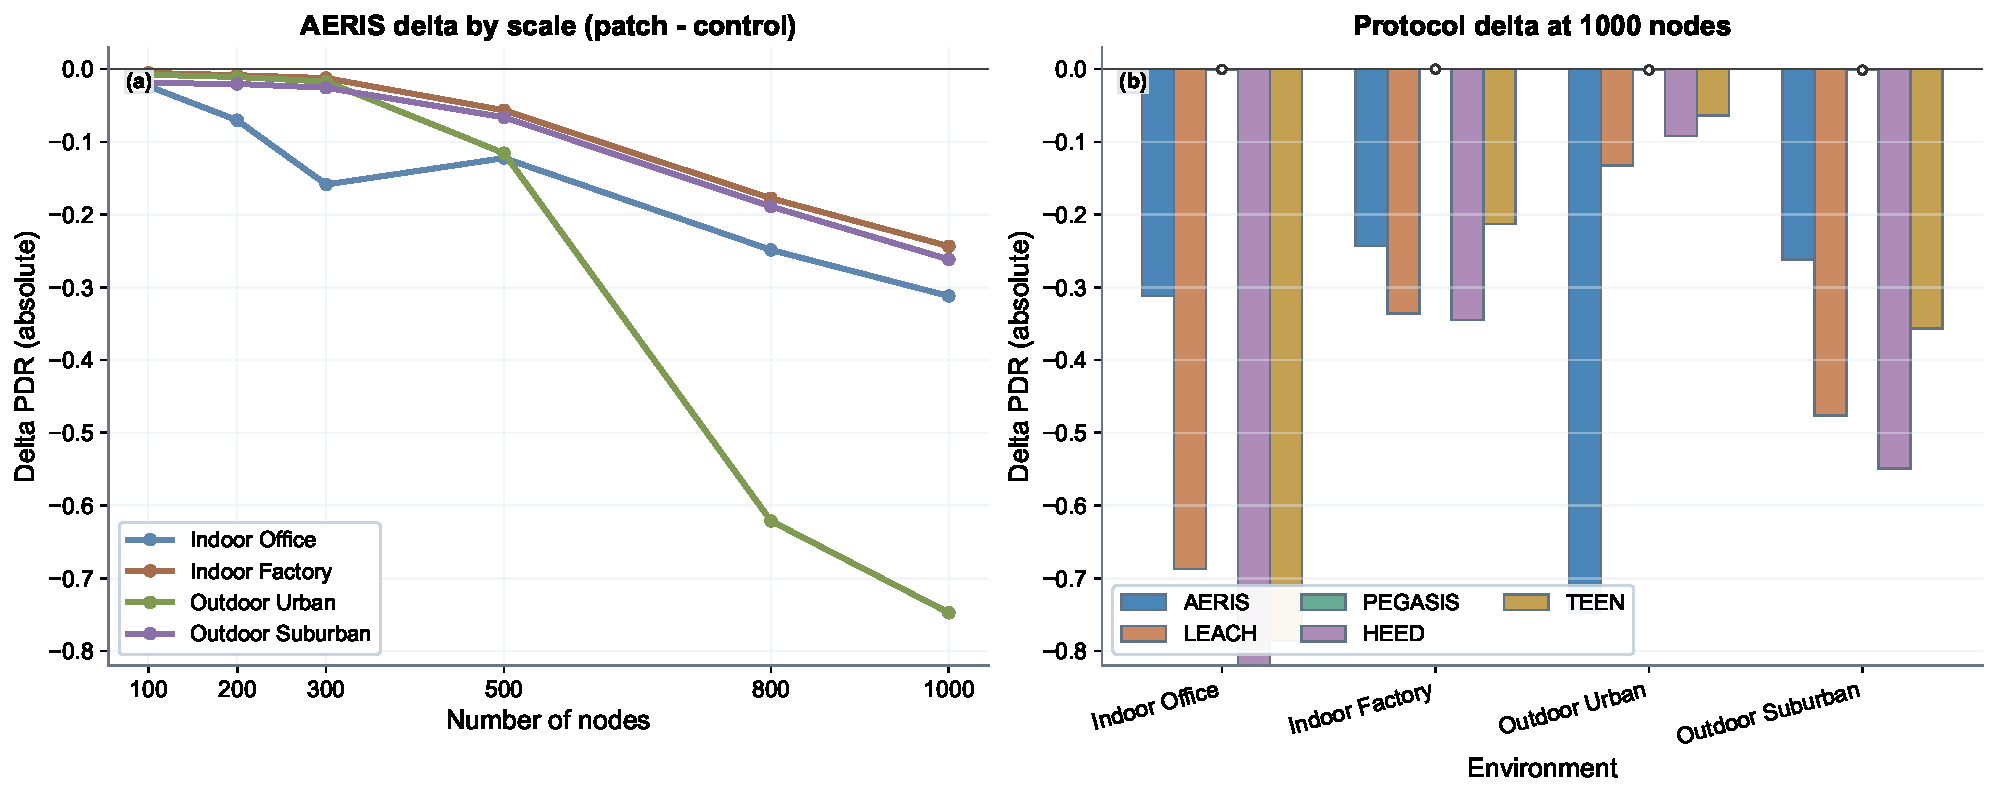
\includegraphics[width=0.99\textwidth]{fig5_s11_patch_control_delta_20260228_s81.pdf}
\caption{Matched stress-comparison evidence. (a) AERIS delta trajectories over node counts (patch - control). (b) Protocol deltas at 1000 nodes across environments. Negative deltas indicate lower PDR under patch mode.}
\label{fig:s11_patch_control}
\end{figure}

At the protocol level, Holm-significant cell counts in the matched stress-comparison block are 24/24 for AERIS, 24/24 for LEACH, 0/24 for PEGASIS, 24/24 for HEED, and 24/24 for TEEN. Together with Figure~\ref{fig:s11_patch_control}, this confirms that the strict patch strongly affects most protocol families, while PEGASIS remains nearly invariant in this matched-delta block. A working technical hypothesis is that the current patch primarily perturbs cluster-based decision points (collision-sensitive parallel uplinks and relay augmentation), whereas PEGASIS uses a serialized chain-forwarding pattern with fewer concurrent uplink competitions in this simulator path; this hypothesis remains subject to explicit code-path instrumentation.

\subsection{Hop-Based Latency and Trade-offs}
At 100 nodes (n=30), AERIS stays near two hops (1.97--1.99), while PEGASIS remains above 31 hops due to chain traversal. LEACH and TEEN show lower average hops because of protocol paths that allow direct-to-BS transmissions.

\begin{figure}[H]
\centering
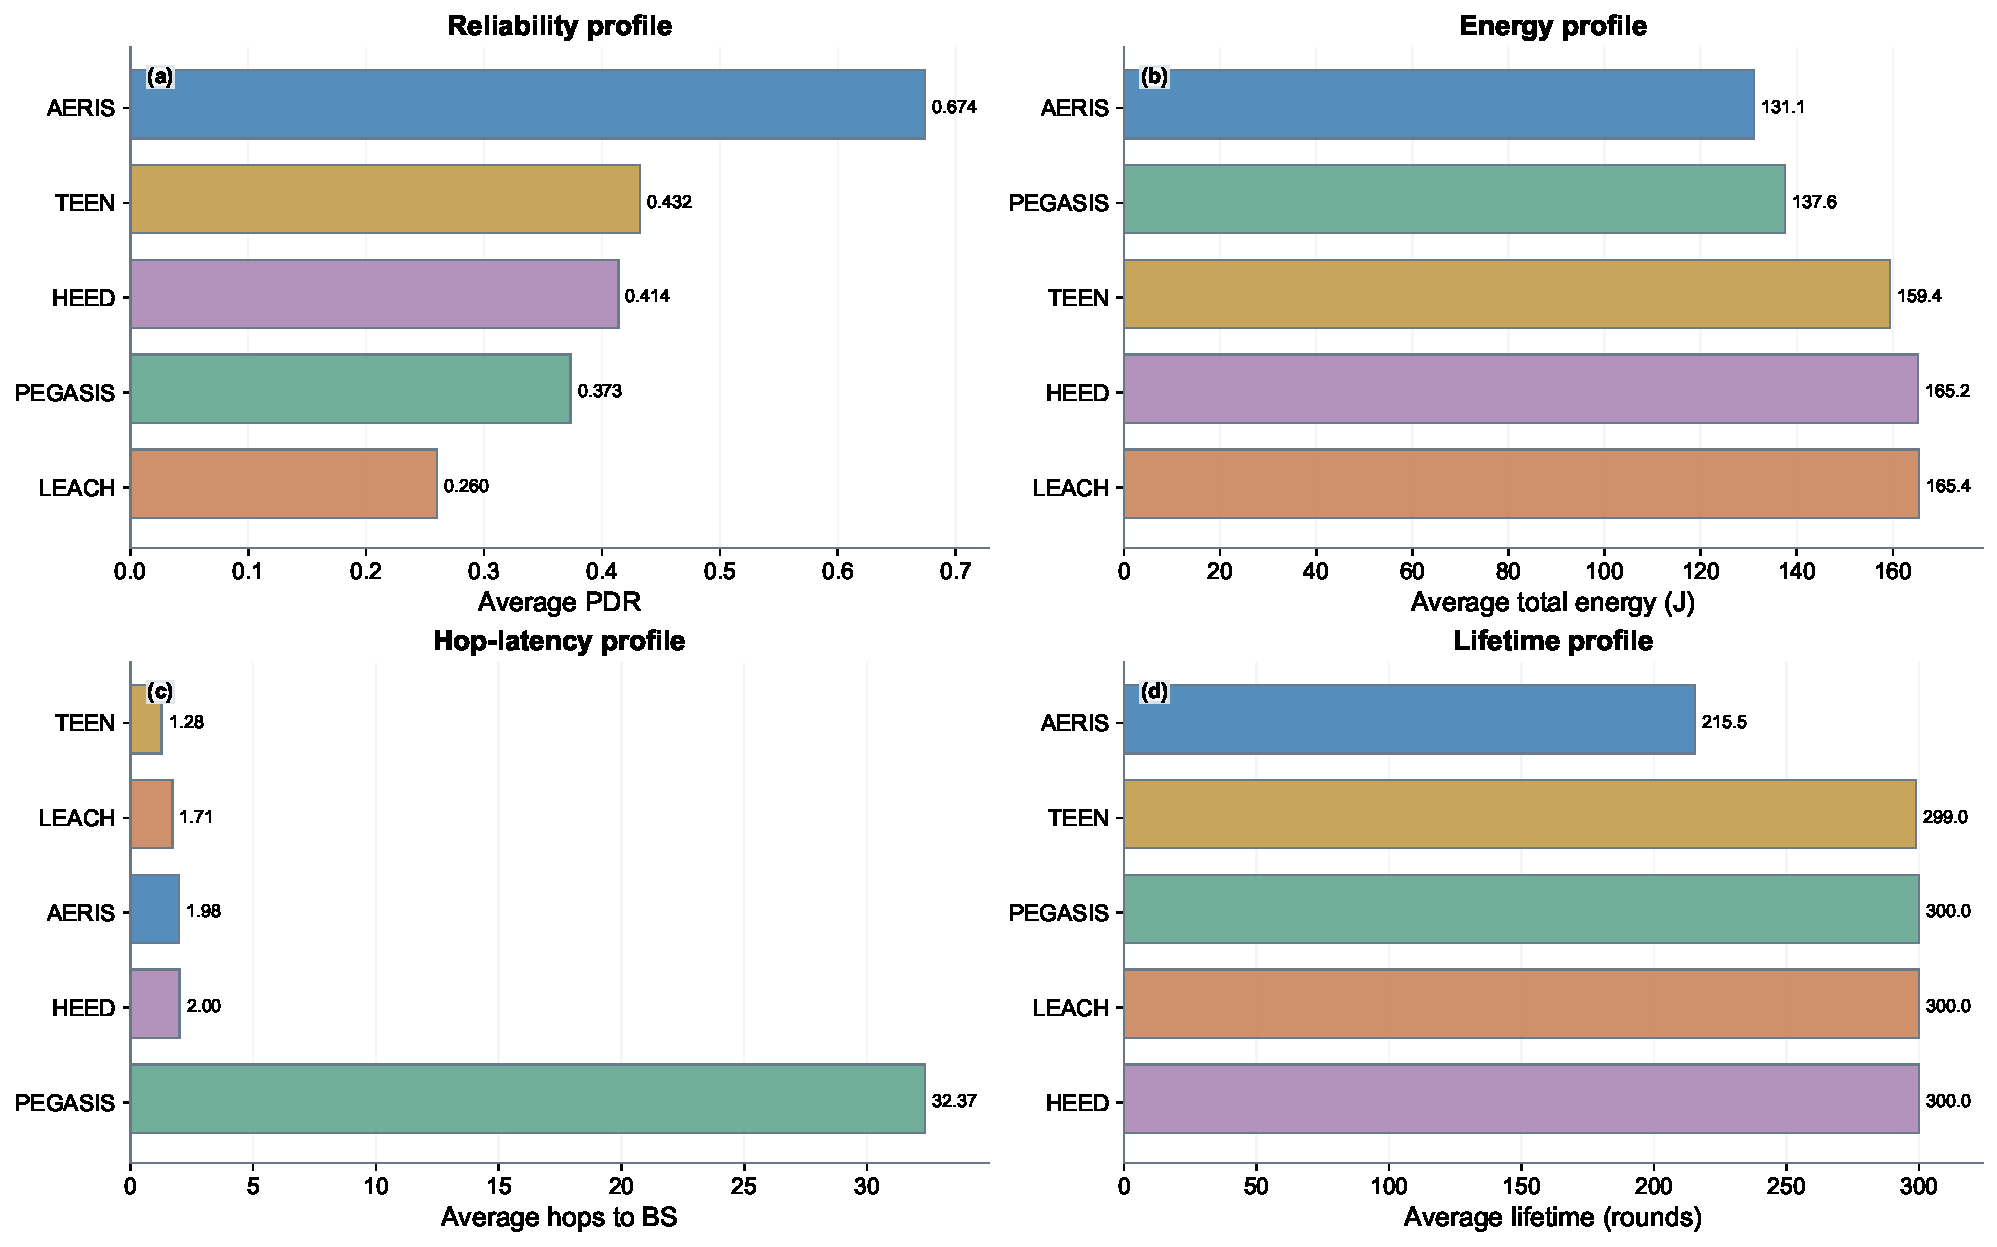
\includegraphics[width=0.99\textwidth]{fig4_tradeoff_panel_20260228_s81.pdf}
\caption{Trade-off panel from publication-tier data: reliability (PDR), energy (J), hop-based latency (average hops), and lifetime (rounds). The hop panel uses a logarithmic x-axis to keep low-hop and high-hop protocols visible in the same frame without overlap.}
\label{fig:tradeoff_panel}
\end{figure}

Figure~\ref{fig:tradeoff_panel} is used as the consolidated reliability-energy-latency-lifetime trade-off view.
\begin{table}[H]
\caption{Energy-focused statistical snapshot from the publication 100-node matrix (pooled across four environments, n=120 per protocol). Delta energy is reported as baseline minus AERIS; positive values indicate higher energy consumption than AERIS.}
\label{tab:energy_snapshot}
\centering
\begin{tabular}{lcccc}
\toprule
Protocol & Avg. energy (J) & Avg. lifetime (rounds) & $\Delta E$ vs AERIS (J) & Holm-corrected $p$ (energy) \\
\midrule
AERIS   & 131.1 & 215.5 & --    & -- \\
LEACH   & 165.4 & 300.0 & +34.4 & $5.27\times10^{-40}$ \\
PEGASIS & 137.6 & 300.0 & +6.5  & $3.99\times10^{-4}$ \\
HEED    & 165.2 & 300.0 & +34.2 & $5.13\times10^{-40}$ \\
TEEN    & 159.4 & 299.0 & +28.4 & $1.34\times10^{-32}$ \\
\bottomrule
\end{tabular}
\end{table}
Table~\ref{tab:energy_snapshot} shows that AERIS remains the lowest-energy protocol in the publication 100-node matrix, while lifetime remains shorter than PEGASIS/LEACH/HEED due to earlier depletion under reliability-oriented forwarding. This clarifies that the energy panel in Figure~\ref{fig:tradeoff_panel} reflects a reliability-energy-lifetime trade-off rather than a single monotonic objective.

\subsection{NS-3 Trend Validation (AERIS vs LEACH, n=30)}
NS-3 validation is used as a cross-platform trend check rather than a numerical-equivalence proof. Formal significance claims in this block remain restricted to AERIS-versus-LEACH. Under aligned multi-environment settings, AERIS is directionally not lower than LEACH in 27 of 28 tested environment-scale cells; the single exception is indoor\_office at 200 nodes (AERIS--LEACH diff $=-0.0004$, not significant). At 100 nodes, significance is confirmed in 3/4 environments (indoor\_factory, outdoor\_urban, outdoor\_suburban), while indoor\_office remains non-significant. In the 300/500-node extension, all eight environment-scale comparisons are significant after Holm correction; with the 800/1000 extension included, non-significance remains confined to indoor\_office at 1000 nodes. Figure~\ref{fig:ns3_trend_panel} also overlays PEGASIS/HEED/TEEN curves for descriptive context only.

\begin{table}[H]
\caption{NS-3 trend-level validation at 100 nodes (AERIS vs LEACH, n=30; metric: mean PDR).}
\label{tab:ns3_trend}
\centering
\begin{tabular}{lccccc}
\toprule
Environment & AERIS & LEACH & Delta & Holm-corrected $p$ & Significance \\
\midrule
indoor\_office    & 0.9202 & 0.9185 & +0.0017 & 1.00 & no \\
indoor\_factory   & 0.6025 & 0.5336 & +0.0690 & $4.23\times10^{-25}$ & yes \\
outdoor\_urban    & 0.2064 & 0.1899 & +0.0165 & $3.41\times10^{-3}$ & yes \\
outdoor\_suburban & 0.7771 & 0.6921 & +0.0850 & $1.94\times10^{-30}$ & yes \\
\bottomrule
\end{tabular}
\end{table}

Table~\ref{tab:ns3_trend} provides the 100-node NS-3 trend snapshot referenced in this subsection.

\begin{figure}[H]
\centering
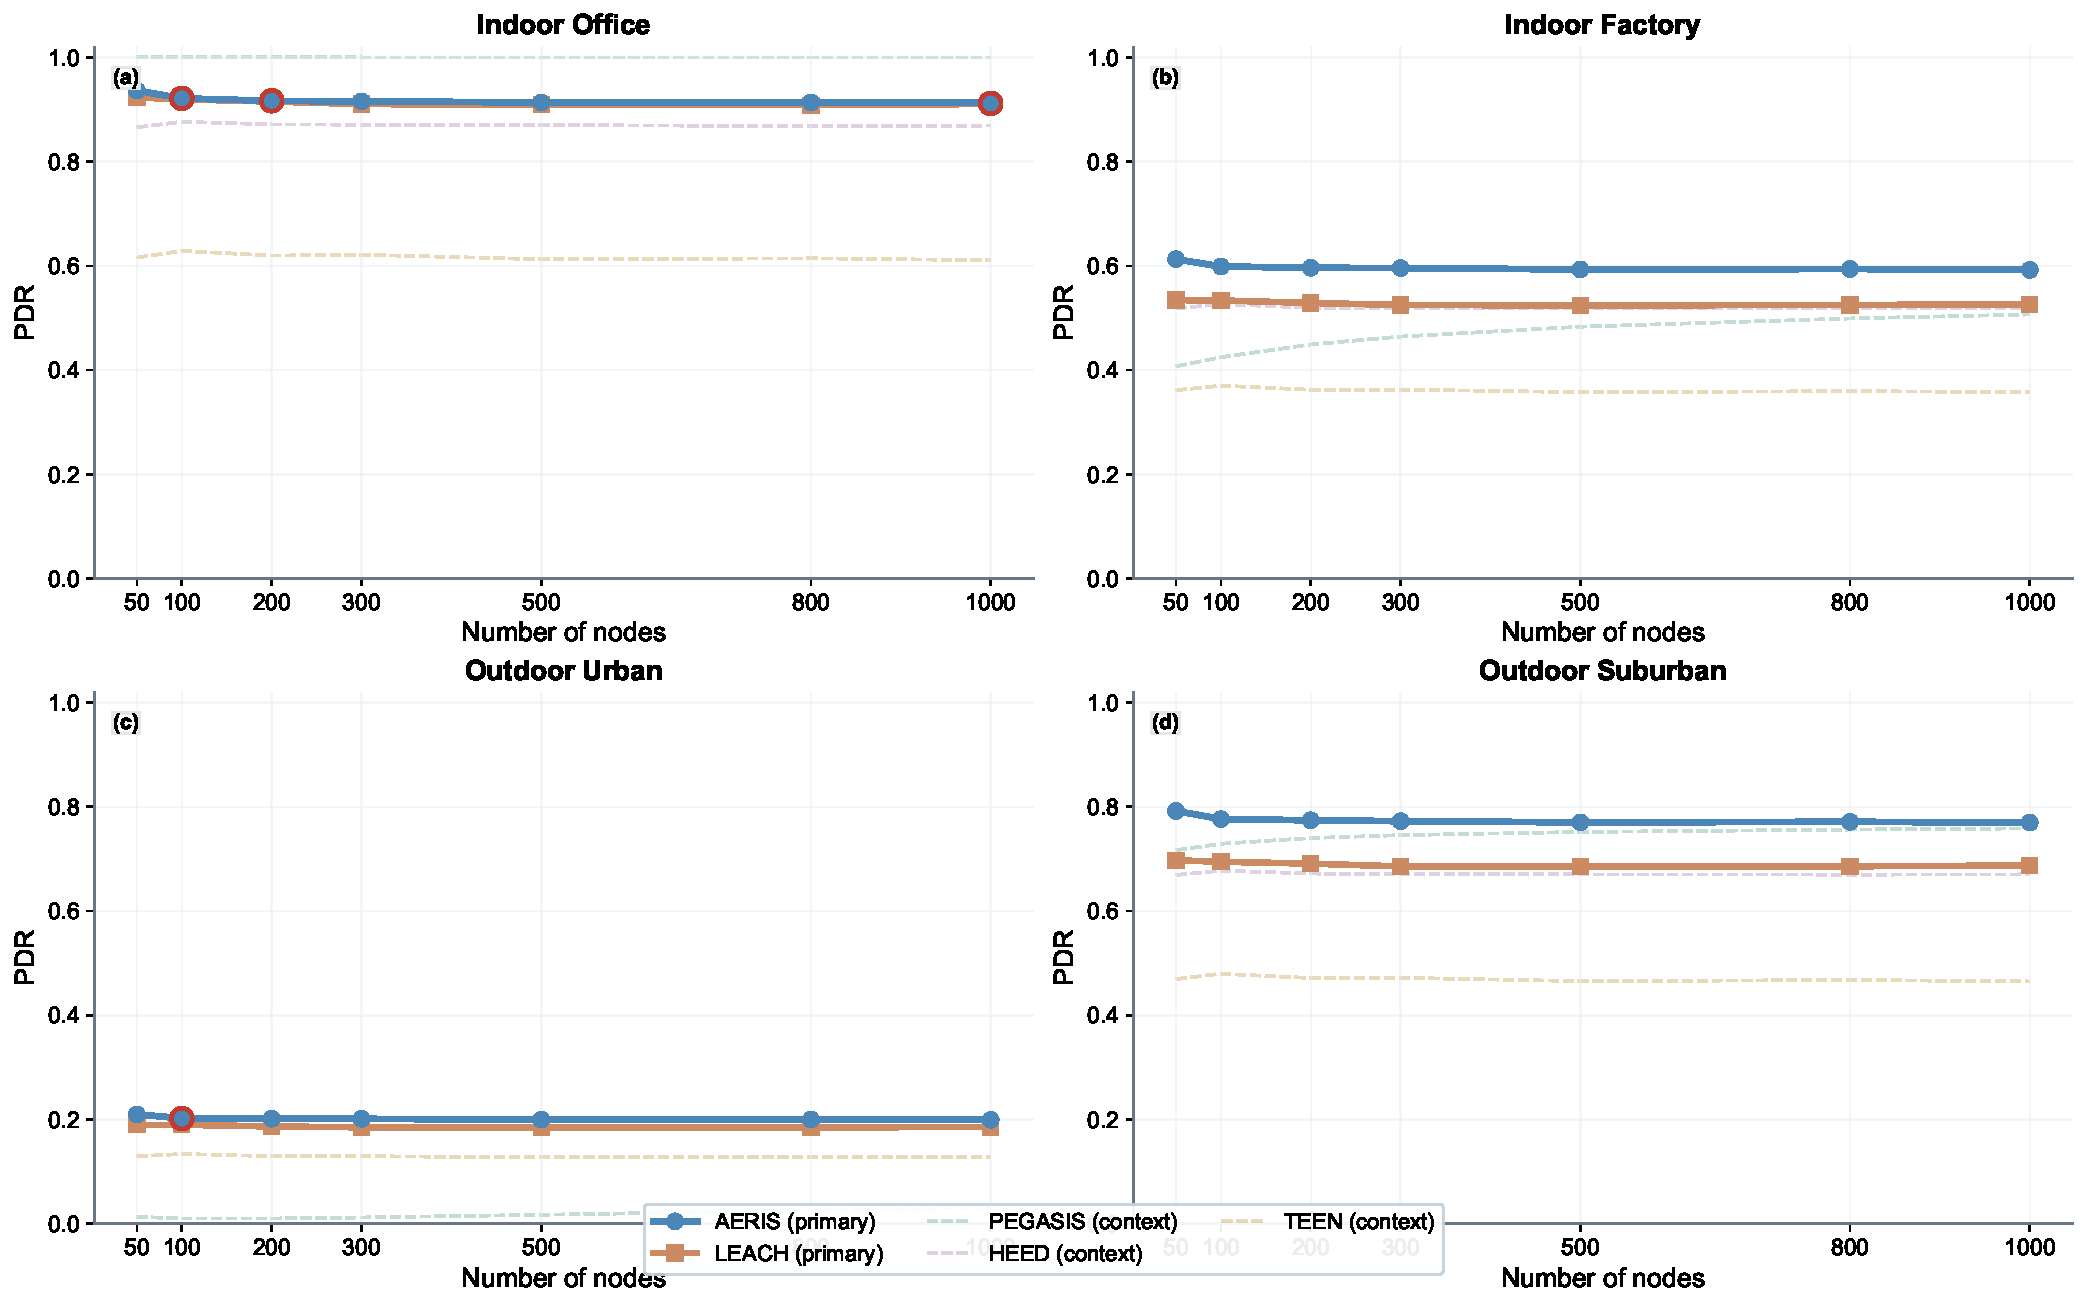
\includegraphics[width=0.99\textwidth]{fig7_ns3_trend_panel_20260228_s81.pdf}
\caption{NS-3 trend validation (50--1000 nodes). Primary inferential pair: AERIS vs LEACH (bold lines, significance markers). PEGASIS/HEED/TEEN are overlaid as descriptive context only (faded lines). Red hollow circles mark Holm non-significant scales for AERIS-vs-LEACH.}
\label{fig:ns3_trend_panel}
\end{figure}

Scope note: this NS-3 block supports trend consistency only. The manuscript does not claim cross-platform numerical equivalence. Across 7 node counts and 4 environments, 25/28 AERIS-versus-LEACH comparisons are significant; the non-significant cells are indoor\_office at node counts 100, 200, and 1000.
Figure~\ref{fig:ns3_trend_panel} visualizes the full 50--1000 node NS-3 trend envelope and the associated significance pattern.

\section{Discussion}
The evidence supports environment-scoped positioning rather than universal superiority. In the reported matrices, AERIS is strongest on reliability in harsh channels.

The manuscript separates three evidence blocks:
\begin{itemize}
\item 100-node multi-environment comparison,
\item primary large-scale matrix (100--1000 nodes) with balanced n=3200 per cell,
\item NS-3 trend validation for AERIS versus LEACH only.
\end{itemize}
Cross-block numerical pooling is avoided because these blocks answer different questions. Under stricter stress-comparison settings (patch minus control), high-scale PDR decreases for most protocols and PEGASIS remains comparatively stable. Under the tx-power sensitivity block, power effects are strong but not globally monotonic. Practical interpretation therefore remains environment-scoped.

An additional boundary is causal interpretation across regime tiers. The difference between the legacy 100-node matrix and the primary large-scale matrix is not interpreted as a single-factor treatment effect, because two changes are introduced together in the primary rerun: (i) strict collision-and-relay physics is enabled, and (ii) previously identified baseline suppressors are removed. For this reason, cross-tier comparisons are used only for scope positioning, while matched stress blocks are used for factor-specific direction checks.

Compared with recent adaptive-routing studies \cite{Ren2024,Okine2024,Naeem2024DRL,Scientific2025DRLGNN,Kaddi2024GWOCSMA,Wang2024Geographic,Tariq2024A,Jain2025Optimized,Ti2026HEOCP,Manogaran2025DDQN}, this work contributes a reproducible large-sample evaluation envelope with explicit regime separation and cross-platform trend checks. Prior studies often report gains in one operating regime (fixed topology, fixed power, or single validation matrix), while this manuscript reports three coupled evidence blocks (ranking matrix, matched degradation matrix, and power-sensitivity matrix) so that ranking gains and absolute reliability penalties are evaluated together. The main distinction is methodological: rather than reporting a single favorable matrix, we report both primary ranking evidence and matched stress/sensitivity blocks that expose when absolute reliability degrades.

Practical interpretation also requires separating statistical and engineering significance. At large sample sizes, very small absolute differences can be significant after correction. For this reason, we interpret each result jointly by corrected $p$ value, effect size, and absolute PDR delta. Energy interpretation is similarly conditioned: lower total energy can co-occur with shorter lifetime when earlier network termination occurs.

\paragraph{Interpretation of Matched Degradation Block.}
The matched stress-confirmation matrix shows that enabling the current patch configuration (MAC-collision plus multihop relay) reduces absolute AERIS PDR in all 24 matched cells. This does not contradict the primary ranking result, because ranking and absolute-level behavior answer different questions: (i) ranking asks whether AERIS remains higher than alternatives under the same strict setting, while (ii) the matched confirmation matrix asks how far the strict patch shifts each protocol relative to its own control path under identical sample sizes. In our data, strict-physics penalties affect all protocols, but the penalty profile is not uniform across protocol families. Therefore, the correct interpretation is not ``AERIS improves under patch'', but ``AERIS keeps relative advantages in harsh regimes while absolute reliability drops under stricter channel/relay assumptions.'' This distinction is central to deployment calibration.

\paragraph{Practical Deployment Guidance.}
Based on the completed matrices, the following deployment guidance is supported by the reported evidence:
\begin{itemize}
\item In harsh environments (indoor\_factory, outdoor\_urban, outdoor\_suburban), enabling Gateway support is recommended because no-gateway ablations reduce reliability.
\item In benign indoor\_office conditions, gains are smaller and model overhead should be justified against application reliability targets.
\item For high-scale deployments, use the primary large-scale matrix as primary evidence and use stress/sensitivity blocks for calibration.
\item Tx-power settings should be environment-tuned; monotonic power assumptions are not supported by the sensitivity block.
\end{itemize}

\begin{table}[H]
\caption{Environment-scoped engineering interpretation from the reported evidence.}
\label{tab:deployment_summary}
\centering
\small
\begin{tabular}{>{\raggedright\arraybackslash}p{0.24\textwidth} >{\raggedright\arraybackslash}p{0.42\textwidth} >{\raggedright\arraybackslash}p{0.26\textwidth}}
\toprule
Environment type & Recommended interpretation & Main caveat \\
\midrule
indoor\_office & Reliability gaps are small at high scale; deployment cost and simplicity can dominate design choice & Some NS-3 cells are non-significant \\
indoor\_factory & AERIS with Gateway support gives the most stable reliability gain & Calibrate tx-power and collision parameters \\
outdoor\_urban & AERIS remains preferable under harsh links in both simulator regimes & High-scale behavior is sensitive to physics settings \\
outdoor\_suburban & AERIS trend remains favorable in simulator and NS-3 trend checks & Do not assume monotonic power-response \\
\bottomrule
\end{tabular}
\normalsize
\end{table}

Table~\ref{tab:deployment_summary} summarizes the actionable interpretation boundaries for deployment decisions.

\paragraph{Validity Notes.}
Three boundaries are explicit in this draft. First, the reported comparisons are simulator-based under the tested channel taxonomy. Second, NS-3 evidence is used for cross-platform trend validation (AERIS vs LEACH), not full five-protocol numerical alignment. Third, module contributions are context dependent: Gateway and CAS effects vary by environment and are not globally monotonic.

\section{Limitations and Future Work}
\begin{itemize}
\item Current evidence is simulation-based under the tested channel taxonomy.
\item NS-3 validation in this manuscript focuses on AERIS versus LEACH; full five-protocol cross-platform ranking is future work.
\item The primary large-scale matrix (n=3200 per cell) includes explicit collision and relay constraints, but does not replace hardware-in-the-loop validation.
\item The stress-comparison matrix (patch minus control), the tx-power sensitivity matrix, and the matched stress-confirmation matrix show that stricter physics assumptions and tx-power changes can materially alter absolute PDR, so deployment requires environment-specific calibration.
\item In the matched stress-confirmation matrix, PEGASIS shows near-invariant patch-minus-control deltas; this behavior is treated as a simulator-coupling artifact requiring dedicated implementation audit. A working technical hypothesis is that serialized chain forwarding exposes fewer branch points to patch toggles than cluster-centric baselines under the current code path. In the primary large-scale ranking matrix, all protocols (including PEGASIS) are executed under the same strict collision-and-relay path without mixing a control arm, so this artifact affects interpretation of the matched stress block but does not alter the standalone primary-matrix ranking values.
\item Reported gains are limited to the tested baseline set and topology families in this manuscript.
\item Hop count is a route-length proxy, not a wall-clock latency benchmark under full MAC scheduling.
\end{itemize}

\section{Conclusion}
AERIS is a reliability-oriented routing option for heterogeneous WSN channels. In the legacy 100-node comparability matrix, it achieves the highest mean PDR within the tested baseline set across all four environments. In the primary large-scale matrix (100--1000 nodes, n=3200 per cell, explicit collision/relay modeling), AERIS is rank-1 in three environments (indoor\_factory, outdoor\_urban, outdoor\_suburban) and rank-2 in indoor\_office where PEGASIS remains dominant.

NS-3 provides trend-level cross-platform support for AERIS versus LEACH. The completed stress and sensitivity blocks show that stricter physics assumptions and tx-power changes materially affect high-scale behavior. In the matched stress-confirmation matrix, AERIS patch-minus-control deltas are negative and significant in all 24 environment-scale cells under the current patch setup.

The practical conclusion is environment-scoped deployment: AERIS remains strong for reliability-first operation in harsh channels, while benign indoor conditions at large scale may favor chain-forwarding baselines. Final parameterization should therefore be environment-tuned using matched stress and sensitivity matrices; for example, the indoor\_factory 500-node cell favors tx10 over tx5/tx15 under the current interference topology.

\authorcontributions{Conceptualization, X.Z. and K.L.; methodology, K.L. and J.L.; software, K.L.; validation, X.Z. and J.L.; writing---original draft preparation, K.L.; writing---review and editing, X.Z.; supervision, X.Z.}
\funding{This research received no external funding.}
\conflictsofinterest{The authors declare no conflict of interest.}
\section*{Data Availability Statement}
The datasets, scripts, manuscript sources, figure-generation code, and provenance sidecar records (including commit identifiers and script hashes) supporting this study are available from the corresponding author and will be released in a versioned public repository upon final publication. The released archive includes the full 100-node benchmark matrix, the primary large-scale matrix and significance tables, stress/sensitivity calibration matrices, and the NS-3 trend-level validation summary.

\reftitle{References}
\bibliography{bibliography}

\end{document}




